% CollaRAG: Graph-Grounded Division of Labor for Multi-Agent Retrieval
% CCF-A Conference Format
\documentclass[11pt,a4paper]{article}

% ===== Core Packages =====
\usepackage[utf8]{inputenc}
\usepackage[T1]{fontenc}
\usepackage{times}
\usepackage{latexsym}
\usepackage{microtype}
\usepackage[margin=2.5cm]{geometry}

% ===== Math & Symbols =====
\usepackage{amsmath}
\usepackage{amssymb}

% ===== Tables & Figures =====
\usepackage{booktabs}
\usepackage{multirow}
\usepackage{graphicx}
\usepackage{subcaption}
\usepackage{xcolor}
\usepackage{colortbl}

% ===== Algorithm =====
\usepackage{algorithm}
\usepackage{algorithmic}

% ===== References =====
\usepackage{natbib}
\usepackage[hidelinks]{hyperref}
\usepackage{url}
\usepackage{placeins}

% ===== Custom Commands =====
\newcommand{\sys}{\textsc{CollaRAG}}
\newcommand{\ie}{\textit{i.e.}}
\newcommand{\eg}{\textit{e.g.}}
\newcommand{\tool}[1]{\texttt{\small #1}}
\newcommand{\best}[1]{\textbf{#1}}
\newcommand{\second}[1]{\underline{#1}}

% ===== Compact Spacing =====
\setlength{\parskip}{0.25em}
\setlength{\parindent}{1em}

\title{CollaRAG: Graph-Grounded Division of Labor \\ for Multi-Agent Retrieval}

\author{
  Anonymous Submission
}

\date{}

\begin{document}
\maketitle

% ===================================================================
% ABSTRACT
% ===================================================================
\begin{abstract}
Existing Retrieval-Augmented Generation (RAG) systems apply a uniform retrieval pipeline to every query, regardless of whether the query calls for a single-fact lookup, multi-hop reasoning, or cross-document synthesis.
This monolithic design forces all queries through the same evidence-gathering procedure, even though no single pipeline can match the evidence shape required by every query type.
We introduce \sys{}, a multi-agent RAG framework built on the principle of graph-grounded division of labor: a triage stage routes each query to a specialist agent whose tool permissions, reasoning protocol, and memory scope match the demand profile of the query, and every routing, reasoning, memory, and capability decision is conditioned on a shared knowledge graph.
Query routing is handled by Intent-Aware Query Triage, a two-level classifier that dispatches each query to the most suitable specialist in a single irreversible step, which replaces the one-pipeline-fits-all bottleneck and enables a clean per-agent ablation.
For multi-hop queries, Graph-Grounded Plan-Execute-Reflect (G-PER) anchors all three reasoning phases to the knowledge graph: the plan is validated against the KG schema before any retrieval budget is spent, execution shares a frontier budget across steps, and reflection checks structural evidence completeness and probes the KG for contradictions, checks that graph-agnostic ReAct and Reflexion cannot perform.
Graph-Grounded Dual-Layer Memory carries experience across queries, with a shared layer that caches evidence subgraphs retrieved by entity-neighborhood overlap rather than by text match and a private layer that stores graph plan templates and typed gap lessons feeding back into G-PER, so that structural learning is separated from cache hits.
Graph-Conditioned Capability Specialization adapts the per-agent tool-permission matrix to the structural footprint of the query on the KG, withdrawing graph-traversal tools and adding a text fallback in graph-poor regions, a mechanism that prior strategy-level routing does not provide.
Five agents, comprising a preprocessor and four task specialists, share a pool of 34 tools that span ten functional categories, and each agent can call only the tools it is permitted to use.
On six QA benchmarks spanning single-hop (NQ, PopQA), multi-hop (HotpotQA, 2WikiMultiHopQA, MuSiQue), and long-form summarization (ASQA) tasks, \sys{} outperforms nine baselines, including the strongest graph-hybrid baseline HippoRAG2~\citep{gutierrez2025hipporag2}, under both the Qwen3-8B and Qwen3-32B backbones.
The largest gains are observed on ASQA ($+7.2$ F1 at Qwen3-8B and $+7.4$ F1 at Qwen3-32B), where no baseline runs a dedicated aggregation pipeline; on the factoid and multi-hop sets, the gains range from $+1.8$ to $+5.7$ F1 (Qwen3-8B) and are driven by intent-aware routing to specialist agents equipped with graph-grounded reasoning and structured reflection.
Ablation studies confirm that intent-aware routing is the single most impactful component, contributing $5.9$--$12.2$ EM points when it is removed.
\end{abstract}

\noindent\textbf{Keywords:} Retrieval-Augmented Generation, Multi-Agent Systems, Query Routing, Multi-hop Reasoning, Division of Labor

% ===================================================================
% 1. INTRODUCTION
% ===================================================================
\section{Introduction}
\label{sec:intro}

% --- 1. LLM Limitations and Motivation for RAG ---

Large language models (LLMs) now perform strongly on a wide range of language understanding and generation tasks~\citep{wei2022chain}.
Despite this success, LLMs suffer from three well-documented limitations that hinder reliable deployment in knowledge-intensive applications.
Knowledge staleness freezes the parametric knowledge of an LLM at its training cutoff, so that the model cannot reflect recent events or updated domain facts.
Hallucination lets an LLM generate fluent yet factually incorrect content, presenting fabricated information that is indistinguishable from genuine knowledge~\citep{gao2024rag_survey}.
Provenance opacity leaves generated answers without source attribution, which makes it impossible for users to verify claims or to trace them back to authoritative evidence.
These shortcomings are especially problematic in enterprise question answering, legal and medical consultation, and scientific literature review, where factual accuracy and traceability are essential.

Retrieval-Augmented Generation (RAG)~\citep{lewis2020rag} has emerged as a leading paradigm for addressing these limitations.
By retrieving relevant passages from an external knowledge base and prepending them to the LLM prompt at inference time, RAG grounds generation in verifiable evidence without retraining the model.
This architecture offers three practical advantages. Knowledge can be updated by modifying the external corpus rather than by retraining billion-parameter models, generated answers can be traced back to specific source passages, which makes the system auditable, and the same LLM can serve multiple domains by swapping the underlying knowledge base.
Supported by mature infrastructure, including vector databases such as FAISS~\citep{johnson2019faiss} and Milvus, embedding models~\citep{chen2024m3embedding}, and orchestration frameworks such as LangChain and LlamaIndex, RAG has become one of the most widely adopted paradigms for deploying LLMs in knowledge-intensive production systems.

% --- 2. Existing RAG Paradigms ---

The standard RAG pipeline follows a sequential four-stage architecture: chunking (splitting documents into passages), indexing (encoding chunks into dense vectors), retrieval (finding the top-$k$ relevant chunks through similarity search), and generation (feeding the retrieved chunks to the LLM for answer synthesis).
Existing RAG methods have advanced the retrieval substrate along three directions:
text-based methods enhance passage retrieval through hierarchical indexing (\eg, RAPTOR~\citep{sarthi2024raptor}) and hybrid dense-sparse fusion;
graph-based methods such as TOG~\citep{sun2024tog} and G-Retriever~\citep{he2024gretriever} exploit entity-relation structures for multi-hop reasoning;
and hybrid methods, including GraphRAG~\citep{edge2024graphrag}, LightRAG~\citep{guo2024lightrag}, and HippoRAG~\citep{gutierrez2024hipporag}, combine textual evidence with graph traversal and achieve the current state of the art on multi-hop QA benchmarks.

% --- 3. Core Limitation: Retrieval Monolithism ---

Yet across all three families, one fundamental design assumption remains unchallenged: every query passes through the same retrieval pipeline.
Whether a user poses a trivial factual question or a complex comparative analysis that requires evidence chains across multiple documents, the system invokes identical retrieval logic, tool budgets, and reasoning strategies.
We call this pattern retrieval monolithism.

% --- 4. Why Monolithic RAG Is Problematic ---

Retrieval monolithism gives rise to three concrete problems.
Simple queries are over-processed: single-hop factual questions that require only a single passage lookup are funneled through sophisticated multi-step pipelines (\eg, the community summarization of GraphRAG or the PageRank traversal of HippoRAG) without any corresponding gain in quality, and in mixed query workloads that comprise factoid, multi-hop, and summarization requests, a substantial fraction of the queries are single-hop and benefit nothing from such machinery.
Complex queries are under-reasoned: multi-hop questions require chaining evidence across multiple documents and often involve entity comparison, temporal reasoning, or causal inference, yet existing methods apply the same retrieval budget regardless of query complexity; even graph-based systems typically perform retrieval in a single forward pass without iterative evidence verification. Once the initial retrieval misses a critical linking entity, most systems therefore lack a mechanism to detect and repair the gap.
Summarization queries are under-aggregated: queries that request overviews or syntheses require global information aggregation across many passages rather than point retrieval of specific facts, yet existing multi-hop QA-oriented RAG systems rarely treat summarization as a first-class routed intent with a dedicated aggregation pipeline; as a result, summarization requests are often handled by the same top-$k$ retrieval mechanism that serves factoid QA, which may cover only a small portion of the relevant corpus and produce incomplete summaries.

These limitations are structural consequences of the monolithic design rather than bugs in individual systems.
Addressing them requires rethinking the retrieval architecture itself.

% --- 5. Core Idea: Division of Labor ---

We take the division of labor principle as our starting point.
In organizational design, a hospital triages patients by symptom severity, routing a headache to general medicine and a fracture to orthopedics.
Each department has specialized equipment and protocols optimized for its patient population, and no hospital sends every patient through the same diagnostic pipeline.
A retrieval system should behave in the same way, routing queries to specialized agents according to query characteristics and equipping each agent with the tools and reasoning strategies best suited to its query type.

% --- 6. Overview of CollaRAG ---

We introduce \sys{}, a framework that replaces the monolithic retrieval pipeline with intent-conditioned specialist execution.
\sys{} routes queries into five handling modes: greeting short-circuit, SingleHop, MultiHop, Summarization, and Other. These modes are supported by a Preprocessor agent and four task-specialist agents.
An intent-aware query triage module classifies incoming queries and dispatches each to the matching handler.
Each task agent draws from a shared pool of 34 tools spanning ten functional categories, with access governed by an adaptive graph-conditioned tool-permission matrix that specializes the toolset of each agent to the structural footprint of the query on the knowledge graph (and that degrades to a static matrix when the graph is unavailable).
The MultiHop agent employs a novel G-PER (graph-grounded Plan-Execute-Reflect) workflow.
A dual-layer memory system enables cross-agent coordination and per-agent progressive learning.

% --- 7. Contributions ---

Specifically, \sys{} makes four technical contributions.

Intent-Aware Query Triage (\S\ref{sec:triage}) proposes a two-level intent classifier that cascades a fast regex-based greeting filter into LLM semantic classification with a keyword-based rule fallback.
The classifier categorizes queries into five handling modes (\texttt{greeting}, \texttt{single\_hop}, \texttt{multi\_hop}, \texttt{summarization}, \texttt{other}) and dispatches each to the matching handler through one-shot deterministic routing.
Unlike prior adaptive retrieval methods, which mainly switch among retrieval depths or strategy templates, our triage operates at the agent level: different intents are handled by specialists with distinct tool permissions, reasoning protocols, synthesis procedures, and private memories.

For multi-hop queries, Graph-Grounded Plan-Execute-Reflect (G-PER, \S\ref{sec:per}) re-grounds the three reasoning phases in the knowledge graph rather than treating the graph as a single optional tool.
Plan emits graph operations (link, traverse, attribute, aggregate) that are validated against the KG schema, which catches malformed steps before any retrieval budget is spent; Execute runs a frontier of pending steps under a shared global budget, which allows an easy step to donate its unused iterations to a harder downstream step; Reflect replaces the scalar quality gate with a structural-completeness check that emits typed evidence gaps ($\texttt{missing\_attribute}$, $\texttt{missing\_path}$, $\texttt{missing\_relation}$) to drive targeted repair, together with an adversarial probe that searches the KG for contradicting relations.
Each mechanism degrades gracefully: in a graph-poor setting, G-PER collapses to text-only PER, which is itself the ablation that isolates the contribution of graph grounding.
This design addresses three weaknesses that flat ReAct loops share with prior plan-and-reflect work~\citep{wang2023plan,shinn2023reflexion}: no commitment to an explicit, schema-validated plan, no principled signal that the gathered evidence is incomplete, and graph-agnostic reasoning.

Across queries, Graph-Grounded Dual-Layer Memory (\S\ref{sec:memory}) maintains two layers of memory with different scopes.
The shared layer caches evidence subgraphs retrieved by entity-neighborhood overlap rather than by text-hash match, which makes reuse reflect the structural recurrence of the same entity neighborhood; this reuse is legitimate on non-repeating benchmarks and is kept separate from the legacy QA cache.
The private layer stores graph plan templates (keyed by compositionality and entity signature and recalled as a plan prior) and typed gap lessons (the output of Reflect in G-PER, fetched pre-emptively before future reasoning), which couples the private layer to the reasoning protocol; a text-only lesson channel, that is, the tool-sequence failures that the Plan of G-PER recalls as avoidance guidance, serves as the graph-poor counterpart, so that the text fallback remains functional.
Such a design separates structural learning from cache hits, which a purely textual memory cannot achieve.

Graph-Conditioned Capability Specialization (\S\ref{sec:capability}) makes the per-agent tool-permission matrix adaptive to the structural footprint of the query on the KG: a cheap, LLM-free probe (entity hit rate, path existence, and density) withdraws graph-traversal tools and adds a text fallback in graph-poor regions, and it collapses the KG projection of a specialist (attribute, path, or community) when the graph cannot support that projection.
This turns a static capability gate into an adaptive, graph-conditioned one and supplies the concrete mechanism, together with a measurable ablation, for the distinction between agent-level and strategy-level routing that prior adaptive-retrieval work~\citep{jeong2024adaptive} only asserts.

% --- 8. Experimental Results ---

We evaluate \sys{} on six QA benchmarks that collectively span three intent types:
single-hop factoid QA (NQ~\citep{kwiatkowski2019nq}, PopQA~\citep{mallen2023popqa}),
multi-hop reasoning (HotpotQA~\citep{yang2018hotpotqa}, 2WikiMultiHopQA~\citep{ho2020constructing}, MuSiQue~\citep{trivedi2022musique}),
and long-form summarization (ASQA~\citep{stelmakh2022asqa}).
This mixed-intent evaluation directly tests the core hypothesis: a system designed for division of labor should excel when queries demand different retrieval strategies.
Using both Qwen3-8B and Qwen3-32B as backbone LLMs, \sys{} achieves the best results across all benchmarks and backbone scales, outperforming the strongest baseline, HippoRAG2~\citep{gutierrez2025hipporag2}, on every dataset, with gains of 5.7 F1 on 2WikiMultiHopQA (Qwen3-8B) and 5.1 F1 on HotpotQA (Qwen3-32B), and the largest gains of 7.2 and 7.4 F1 on ASQA (Qwen3-8B and Qwen3-32B), where the dedicated Summarization agent has no baseline counterpart.
Ablation studies confirm that intent-aware routing is the single most impactful component: removing it causes a drop of $11.7$ EM on 2WikiMultiHopQA, which validates the division-of-labor hypothesis.

% ===================================================================
% 2. RELATED WORK
% ===================================================================
\section{Related Work}
\label{sec:related}

% --- 2.1 Text-Based RAG and Retrieval-Augmented Summarization ---
\subsection{Text-Based RAG and Retrieval-Augmented Summarization}

RAG~\citep{lewis2020rag} established the retrieve-then-generate paradigm, pairing parametric LLMs with non-parametric passage retrieval to ground generation in external evidence, an idea anticipated by retrieval-augmented pre-training such as REALM~\citep{guu2020realm}.
Many vanilla RAG implementations rely on DPR-style bi-encoder retrieval~\citep{karpukhin2020dpr} for open-domain QA, and Fusion-in-Decoder~\citep{izacard2021leveraging} scaled this approach to the parallel processing of many retrieved passages; late-interaction retrieval~\citep{khattab2020colbert} later sharpened matching by comparing query and passage tokens directly.
Subsequent work has refined the retrieval stage along multiple dimensions:
hybrid retrieval that combines dense and sparse (BM25~\citep{robertson2009bm25}) signals through reciprocal rank fusion~\citep{cormack2009reciprocal};
cross-encoder reranking~\citep{nogueira2019passage} for more precise relevance estimation;
and query rewriting~\citep{ma2023query} to bridge the vocabulary gap between queries and documents.
RAPTOR~\citep{sarthi2024raptor} organizes retrieval through recursive abstractive trees, which enables retrieval at multiple levels of abstraction, and the retrieval unit itself can be refined: indexing propositions in place of fixed passages improves both retrieval and downstream QA~\citep{chen2024densex}.
These methods enhance retrieval quality, but they apply a uniform pipeline to all queries regardless of complexity, which is the monolithic limitation that \sys{} addresses.

While most RAG systems focus on factoid QA, real-world queries often demand summarization or synthesis across many passages.
The Map-Reduce paradigm for distributed text processing~\citep{dean2008mapreduce} has been adapted to LLM-based summarization: each passage is summarized independently (Map), and the summaries are then aggregated into a coherent overview (Reduce).
Simply retrieving more passages does not solve the problem: language models use long contexts unevenly and degrade when relevant evidence falls in the middle of a long input~\citep{liu2024lostmiddle}, which makes principled aggregation, rather than retrieval depth, the real bottleneck for synthesis queries.
GraphRAG~\citep{edge2024graphrag} uses community-level summaries for global queries but does not provide a dedicated summarization agent.
Existing RAG surveys~\citep{gao2024rag_survey, zhao2024retrieval} identify summarization as an underserved query type in current systems.
\sys{} addresses this gap with a dedicated Summarization agent that implements a full Map-Reduce pipeline, comprising broad retrieval ($k\!=\!50$), per-chunk LLM summarization, and final aggregation.
This makes summarization a first-class routed intent within the same multi-agent RAG framework, rather than an external summarization chain or a generic retrieval mode.

% --- 2.2 Graph-Based RAG and Multi-Hop Reasoning ---
\subsection{Graph-Based RAG and Multi-Hop Reasoning}

Knowledge graphs provide structured pathways for multi-hop reasoning.
GraphRAG~\citep{edge2024graphrag} performs community detection on entity graphs using the Louvain algorithm~\citep{blondel2008louvain} and generates hierarchical summaries for query-focused retrieval.
LightRAG~\citep{guo2024lightrag} introduces dual-level (key-entity and high-level topic) graph retrieval for improved efficiency.
TOG~\citep{sun2024tog} uses LLMs to iteratively traverse knowledge graph triples, G-Retriever~\citep{he2024gretriever} integrates graph neural networks with LLMs for subgraph retrieval, and Reasoning-on-Graphs~\citep{luo2024rog} plans explicit relation paths before retrieval so that the reasoning chain remains inspectable.
HippoRAG~\citep{gutierrez2024hipporag} draws on hippocampal indexing theory, implementing personalized PageRank over a knowledge graph to mimic human associative memory, and HippoRAG2~\citep{gutierrez2025hipporag2} extends this design with deeper memory integration and passage-level retrieval.
These systems optimize what is retrieved by enriching the knowledge substrate, yet they do not adapt how retrieval is orchestrated according to query type, which is an orthogonal dimension that \sys{} addresses through intent-aware routing.
\sys{} is complementary to these retrieval substrates: graph traversal, dense retrieval, and hybrid retrieval can all serve as tools inside the specialist agents.

On the reasoning side, multi-hop QA requires chaining evidence across multiple passages.
Chain-of-thought prompting~\citep{wei2022chain} enables LLMs to articulate intermediate reasoning steps.
IRCoT~\citep{trivedi2023ircot} interleaves retrieval with chain-of-thought steps, using each reasoning step to guide the next retrieval query, and achieves strong results on HotpotQA, 2Wiki, and MuSiQue.
Self-Ask~\citep{press2023measuring} and Least-to-Most prompting~\citep{zhou2023leasttomost} decompose complex questions into simpler sub-questions that can be answered sequentially.
Plan-and-Solve~\citep{wang2023plan} generates explicit plans before execution.
These methods improve multi-hop reasoning within a single pipeline.
The MultiHop agent of \sys{} builds on these ideas but introduces a structural innovation: each of the plan, execute, and reflect phases is grounded in the knowledge graph.
The plan is schema-validated, execution shares a frontier budget, and reflection checks structural evidence completeness and probes for graph-level contradictions, so that the reasoning protocol exploits graph structure that text-only plan-and-reflect methods~\citep{wang2023plan,shinn2023reflexion} cannot access.

% --- 2.3 Adaptive, Agentic, and Memory-Augmented RAG ---
\subsection{Adaptive, Agentic, and Memory-Augmented RAG}

Recent work has begun to challenge the one-size-fits-all assumption.
Self-RAG~\citep{asai2024selfrag} trains an LLM to decide when to retrieve and to self-critique generated outputs using reflection tokens, but it applies the same retrieval mechanism once retrieval is triggered.
Adaptive-RAG~\citep{jeong2024adaptive} trains a query-complexity classifier (on T5-Large) to route among three strategies, that is, no retrieval, single-step retrieval, and multi-step retrieval.
CRAG~\citep{yan2024crag} evaluates retrieval quality and triggers corrective web searches when confidence is low.
These approaches adapt retrieval decisions at the strategy level (whether to retrieve, how many retrieval steps to take, and whether to correct retrieval results), yet they route to pre-defined strategies within a single pipeline.
FLARE~\citep{jiang2023flare} triggers retrieval actively when the generation confidence of the LLM drops, but applies a uniform retrieval mechanism once retrieval is triggered.
StructRAG~\citep{li2024structrag} selects a knowledge structure (table, graph, or catalogue) conditioned on the task type, which is adjacent to our triage but operates at the representation level rather than at the agent level.
KAG~\citep{liang2024kag} augments generation with logical-form reasoning over a KG, sharing our emphasis on graph-grounded retrieval but without intent-aware routing or per-agent capability specialization.
\sys{} performs routing at the agent level: the selected handler differs not only in retrieval depth but also in tool permissions, reasoning protocol (single-phase ReAct vs.\ G-PER vs.\ Map-Reduce), memory scope, and synthesis procedure, thereby realizing a true division of labor rather than a strategy-selection switch.

The rise of LLM-based agents~\citep{xi2023rise} has introduced tool use into RAG.
ReAct~\citep{yao2023react} interleaves reasoning and action (tool invocation) in a single loop.
Toolformer~\citep{schick2023toolformer} teaches LLMs to decide when and how to call external tools.
Multi-agent frameworks such as MetaGPT~\citep{hong2024metagpt} and AutoGen~\citep{wu2024autogen} enable multiple agents to collaborate through conversational protocols.
These multi-agent systems, however, assume that agents need to negotiate by exchanging messages, debating solutions, or voting on outcomes.
\sys{} instead adopts a dispatch model: a classifier makes a one-shot routing decision, and the assigned specialist agent executes independently, with no dialogue between agents.
This design prioritizes deterministic reproducibility and clean ablation boundaries over emergent collaboration, while still achieving the benefits of specialization through the tool-permission matrix.

Standard RAG systems are stateless: each query is processed independently, with no memory of past interactions.
MemGPT~\citep{packer2023memgpt} mitigates this by treating the context window as virtual memory and paging information between storage tiers.
HippoRAG~\citep{gutierrez2024hipporag} introduced biologically inspired long-term memory into RAG through knowledge-graph-based indexing.
MemoRAG~\citep{qian2025memorag} builds a global memory model that recalls query-specific clues to guide retrieval over long contexts.
ExpeL~\citep{zhao2024expel} demonstrates that LLM agents can learn from accumulated experience, extracting insights from past task trajectories to improve future performance, while generative agents~\citep{park2023generative} maintain a stream of observations retrieved by recency and importance to ground long-horizon behavior.
Reflexion~\citep{shinn2023reflexion} stores verbal self-reflections as episodic memory to prevent the repetition of mistakes, and Self-Refine~\citep{madaan2023selfrefine} shows that self-generated feedback alone can iteratively improve a draft without additional training.
\sys{} contributes a dual-layer memory architecture that separates cross-agent shared memory (a graph-grounded evidence-subgraph overlap cache, together with the legacy text-hash QA cache, routing statistics, and entity aliases) from per-agent private experiential memory (graph plan templates, typed gap lessons, and tool-sequence lessons).
This separation enables both collaborative knowledge sharing and isolated experiential learning, with clean ablation boundaries between the two layers.

% ===================================================================
% 3. METHOD
% ===================================================================
\section{Method}
\label{sec:method}

\sys{} is built on a single thesis: a retrieval system should not push every query through the same pipeline, because queries differ in the amount of evidence they require, the shape of reasoning they demand, and the kind of aggregation they need.
We realize this thesis as an orchestrator that, for each query, decides which specialist should handle it, equips that specialist with a bounded set of tools, and lets it follow a protocol matched to the query type.
Figure~\ref{fig:pipeline} sketches the end-to-end flow.
In sequence, a query passes through six stages: intent classification, a greeting short-circuit, memory lookups (a text-hash QA cache and a graph-grounded evidence-subgraph overlap cache), query preprocessing, dispatch to one of four task-specialist agents, and post-processing that writes back to memory.
The four contributions of this paper sit at the decision points of this flow: how a query is routed (\S\ref{sec:triage}), how the hardest queries are reasoned about (\S\ref{sec:per}), how experience accumulates across queries (\S\ref{sec:memory}), and how the capability of each specialist is conditioned on the graph (\S\ref{sec:capability}).

\begin{figure*}[t]
\centering
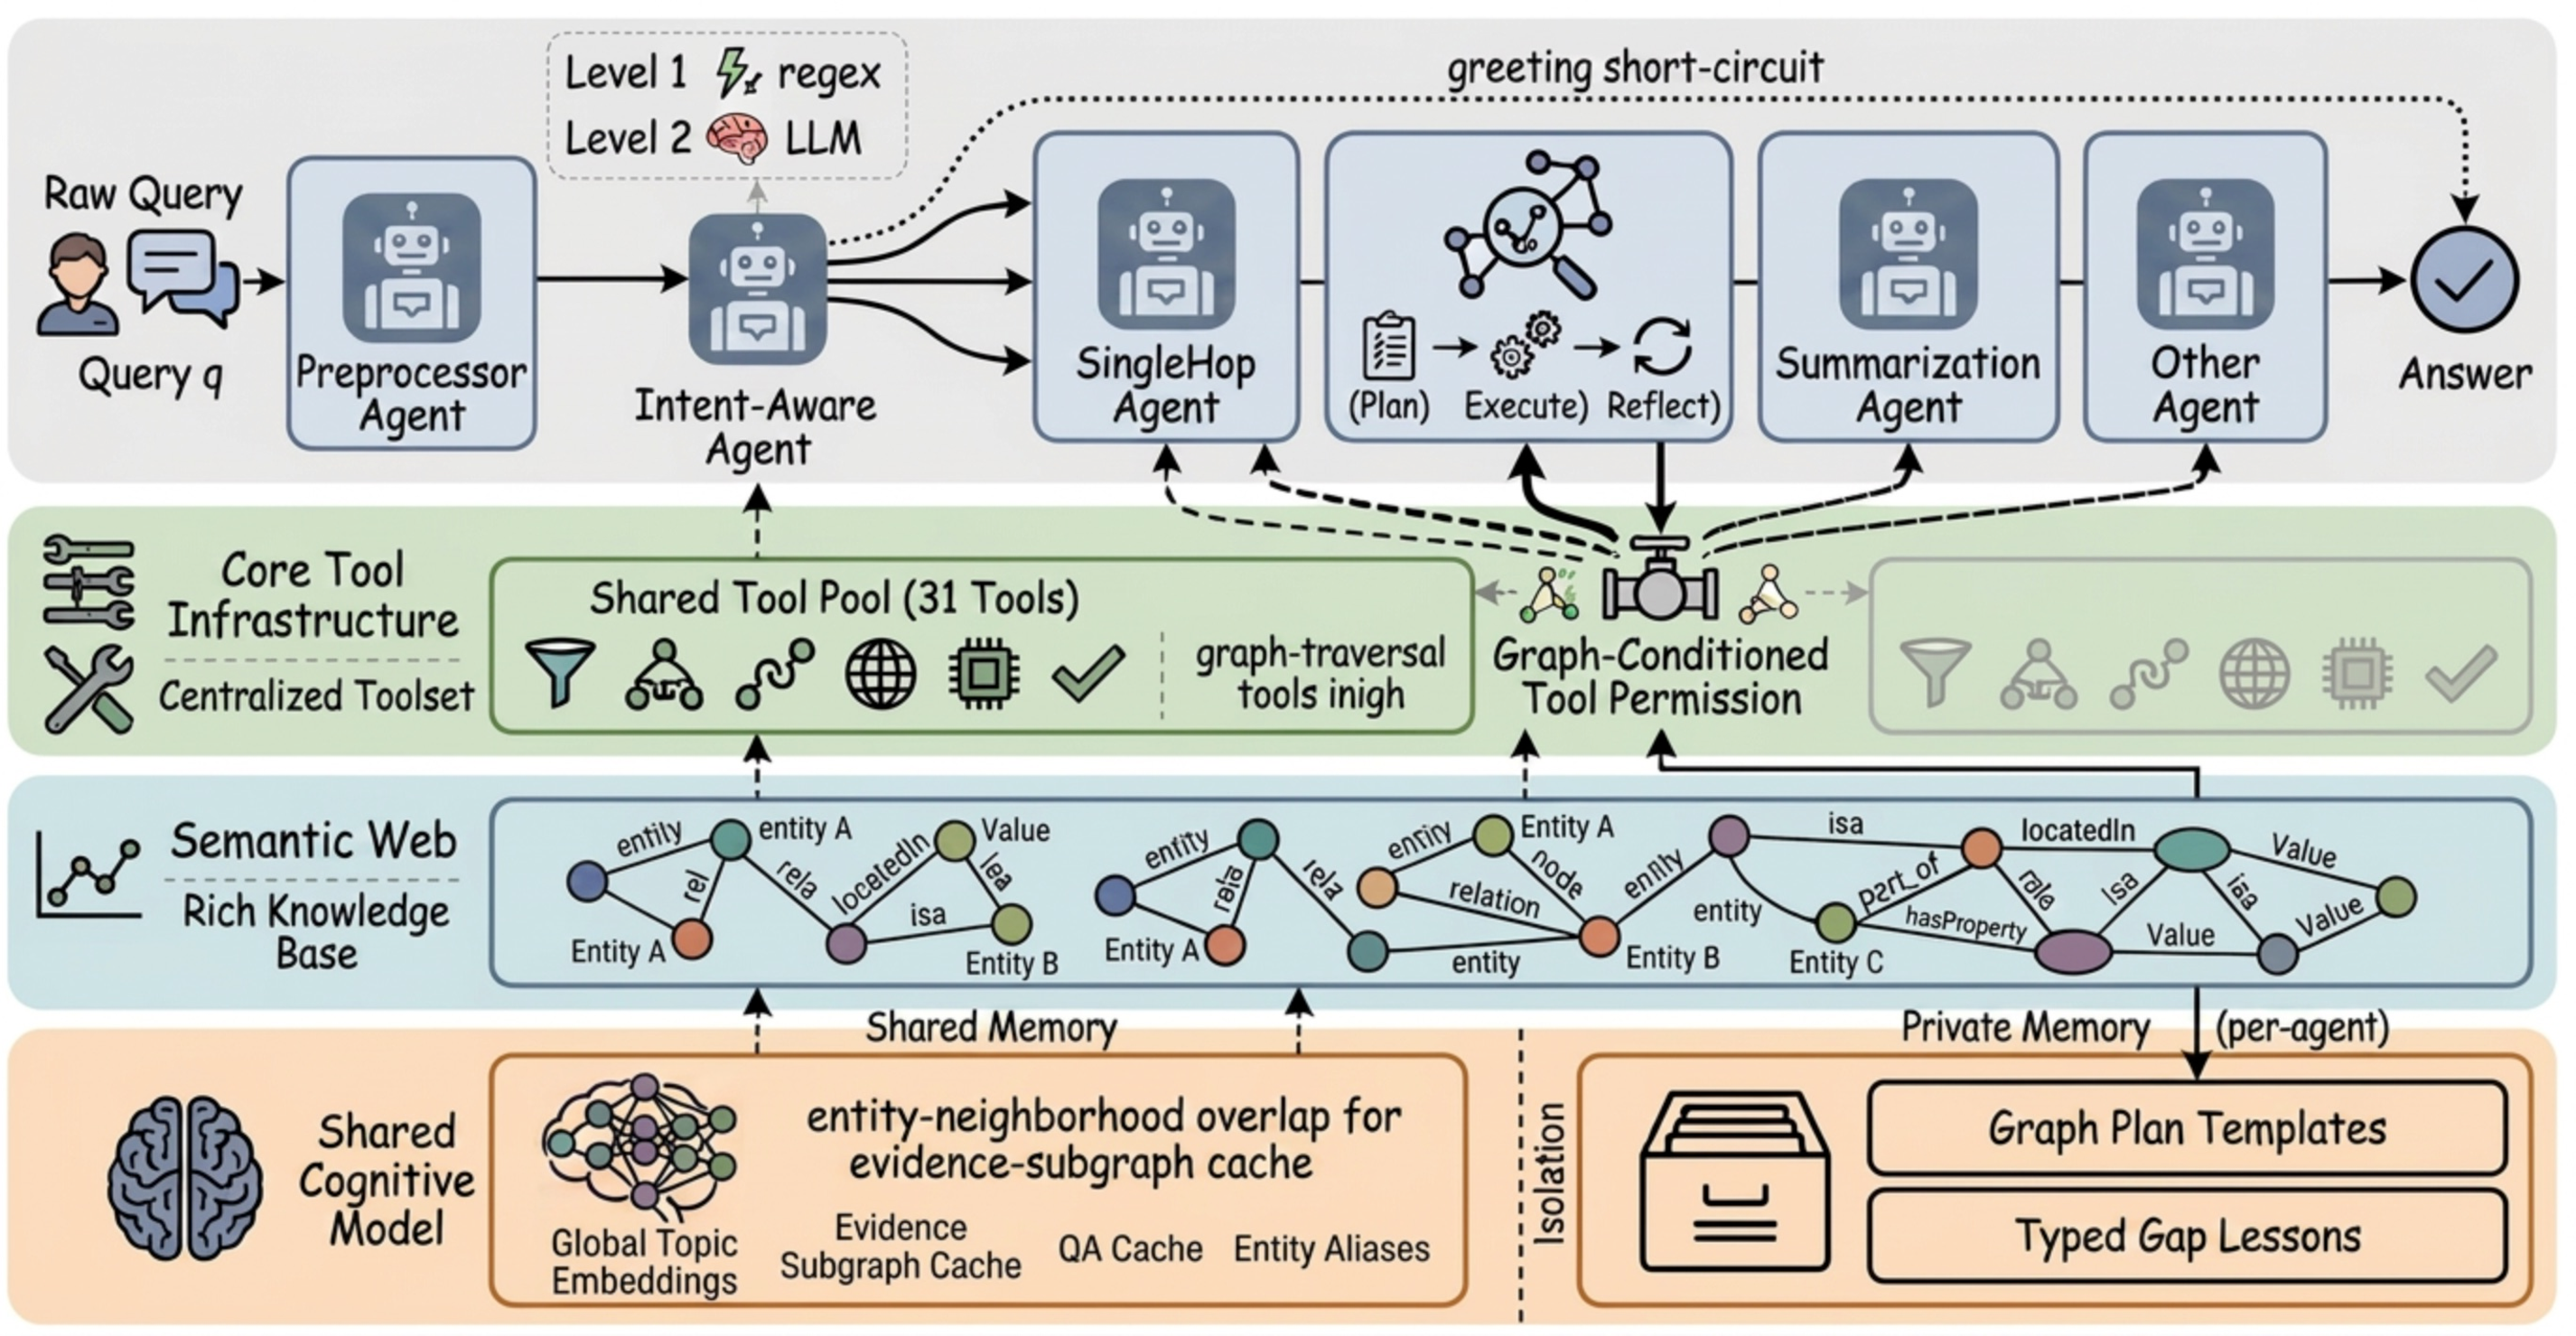
\includegraphics[width=0.96\textwidth]{figures/fig_arch.pdf}
\caption{Architecture of \sys{}. A query is triaged and dispatched in one shot to a specialist agent; the MultiHop agent reasons through G-PER (Plan, Execute, Reflect); the toolset of each agent is gated by the graph footprint of the query; and a graph-grounded dual-layer memory underlies all agents and is fed by the Reflect phase of G-PER.}
\label{fig:pipeline}
\end{figure*}

% -------------------------------------------------------------------
% 3.1 Intent-Aware Query Triage
% -------------------------------------------------------------------
\subsection{Intent-Aware Query Triage}
\label{sec:triage}

The triage module answers one question per query: which specialist should run?
It is a two-level cascade rather than a single classifier, because greetings are trivially detectable and should never incur the cost of a semantic LLM call.
Level~1 is a regex filter for greeting patterns; a hit returns a direct LLM response and skips the rest of the pipeline.
Level~2 sends the non-greeting query to the backbone LLM, which returns one of four labels, namely \texttt{single\_hop}, \texttt{multi\_hop}, \texttt{summarization}, or \texttt{other}, and a keyword-rule fallback covers parse failures (summarization and comparative keywords, otherwise \texttt{single\_hop}).
The full classification prompt is given in Appendix~\ref{app:prompt_classify}.
Formally, the routing decision is
\begin{equation}
a^{*}(q)=
\begin{cases}
\text{greet}, & \text{if } L_{1}(q)=\text{greet},\\[2pt]
\mathrm{dispatch}\!\bigl(L_{2}(q)\bigr), & \text{otherwise},
\end{cases}
\quad a^{*}\in\{\text{SH},\text{MH},\text{SM},\text{OT}\}\cup\{\text{greet}\},
\label{eq:route}
\end{equation}
where $L_{1}$ short-circuits greetings and $L_{2}$ labels the rest.
Routing is one-shot and irreversible: once $a^{*}$ is chosen, the query stays with that agent.
We impose this constraint deliberately: it lets us measure the marginal contribution of each specialist cleanly (\S\ref{sec:results}) and prevents a single misclassification from cascading through re-routing.

\paragraph{Four task specialists.}
Each label selects an agent whose protocol fits the demand profile of the query.
All four specialists execute as ReAct agents~\citep{yao2023react} that interleave reasoning and tool calls, observing the result of each call before deciding the next action; MultiHop additionally wraps its ReAct execution inside the graph-grounded Plan and Reflect phases of G-PER (\S\ref{sec:per}), whereas SingleHop, Summarization, and Other run a single-phase ReAct loop suited to their simpler evidence needs.
SingleHop typically converges after one round of hybrid (dense~+~BM25) retrieval that fuses the two rank lists by reciprocal rank fusion,
\begin{equation}
s(d)=\sum_{i\in\{\text{vec},\text{bm25}\}}\frac{1}{\mathrm{rank}_{i}(d)+k},
\label{eq:rrf}
\end{equation}
optionally reranks the fused list, and stops once the retrieved evidence passes a quality check; this is the cheapest path and is sufficient for a single-fact lookup (prompt template in Appendix~\ref{app:prompt_singlehop}).
MultiHop runs the G-PER workflow of \S\ref{sec:per}.
Summarization retrieves a broad pool ($k\!=\!50$), summarizes each passage locally, and reduces the summaries into one overview, which is a shape of aggregation that no factoid-retrieval pipeline provides (Appendix~\ref{app:prompt_summarization}).
Other falls back to web search with optional local retrieval for out-of-domain queries.
A Preprocessor agent then rewrites the query (expansion, coreference resolution, and follow-up merging) after triage and before dispatch; it holds no retrieval tools and only cleans the query text (prompt templates in Appendix~\ref{app:prompt_preprocess}).

\paragraph{Tool-permission matrix.}
All five agents share one pool of 34 tools, but each agent sees only a curated subset (Table~\ref{tab:tool_matrix}).
The matrix is the infrastructure-level enforcement of specialization: MultiHop alone can call graph path search, sub-query decomposition, and claim decomposition, while SingleHop works with a focused 15-tool set.
This prevents a nominally specialized agent from quietly behaving like a generalist.
The complete tool inventory with per-tool descriptions is listed in Appendix~\ref{app:tools}.

\begin{table}[t]
\centering
\small
\begin{tabular}{@{}lccccc@{}}
\toprule
\textbf{Tool Category} & \textbf{PP} & \textbf{SH} & \textbf{MH} & \textbf{SM} & \textbf{OT} \\
\midrule
Retrieval (6)           & 0 & 4 & 6 & 4 & 1 \\
Entity (3)              & 0 & 2 & 3 & 1 & 1 \\
Reasoning (3)           & 0 & 2 & 3 & 1 & 0 \\
Preprocessing (3)       & 3 & 0 & 0 & 0 & 0 \\
Memory (6)              & 3 & 4 & 6 & 4 & 3 \\
Web (2)                 & 0 & 0 & 0 & 0 & 2 \\
IO (2)                  & 0 & 2 & 2 & 2 & 2 \\
Verification (3)        & 0 & 1 & 3 & 1 & 0 \\
Graph Analysis (2)      & 0 & 0 & 2 & 0 & 0 \\
Evidence (4)            & 0 & 2 & 4 & 3 & 1 \\
\midrule
\textbf{Total}          & 6 & 17 & 29 & 16 & 10 \\
\bottomrule
\end{tabular}
\caption{Tool-permission matrix. PP denotes the Preprocessor, SH SingleHop, MH MultiHop, SM Summarization, and OT Other. The Memory category comprises three read tools and three write tools; write access is granted to the specialists that produce the corresponding data. The MultiHop agent holds the broadest toolset (29 of the 34 tools), which reflects its need for graph traversal, sub-query decomposition, relation extraction, and claim decomposition.}
\label{tab:tool_matrix}
\end{table}

% -------------------------------------------------------------------
% 3.2 Graph-Grounded Plan-Execute-Reflect (G-PER)
% -------------------------------------------------------------------
\subsection{Graph-Grounded Plan-Execute-Reflect (G-PER)}
\label{sec:per}

Multi-hop queries are the hardest case: the answer depends on a chain of facts spread across passages, and a single retrieval pass usually returns one link of that chain without the others.
A flat ReAct loop~\citep{yao2023react} interleaves thought and action greedily, which never commits to an explicit plan, has no principled way to notice that the evidence is incomplete, and is graph-agnostic; it treats the knowledge graph as one optional tool among many, which leaves the structure formed by multi-hop evidence invisible to the reasoning protocol.
We re-ground each phase in the knowledge graph and call the result G-PER: Plan emits graph operations that are validated against the KG schema, Execute allocates a shared budget across a frontier of pending steps, and Reflect checks structural evidence completeness and probes the KG for contradictions.
Figure~\ref{fig:per} sketches the resulting protocol.
Every graph-grounded mechanism degrades gracefully: when the graph store is absent or sparse (the graph-poor setting), G-PER collapses to text-only PER, which is itself the ablation that isolates the contribution of graph grounding (\S\ref{sec:ablation}).
The full prompt templates for each phase are given in Appendix~\ref{app:prompt_multihop}.

\begin{figure}[t]
\centering
\includegraphics[width=0.94\columnwidth]{figures/fig_gper.pdf}
\caption{G-PER: graph-grounded Plan-Execute-Reflect. Plan is schema-constrained, Execute is frontier-based, and Reflect is structural and adversarial.}
\label{fig:per}
\end{figure}

\paragraph{Plan (schema-constrained).}
Given $q$, the LLM produces a retrieval plan as a bounded list of graph operations rather than free-text sub-queries:
\begin{equation}
P=\bigl[(op_{i},e_{i},r_{i},t_{i})\bigr]_{i=1}^{n},\qquad op_{i}\in\{\textsf{link},\textsf{traverse},\textsf{attribute},\textsf{aggregate}\},\quad n\le n_{\max}{=}5,
\label{eq:plan}
\end{equation}
where $e_i$ is an entity, $r_i$ a relation type, and $t_i$ a target entity.
Before any retrieval budget is spent, each step is validated against the KG schema:
\begin{equation}
V(s_i)=\bigl(r_i\in\mathcal{S}\cup\{\bot\}\bigr)\wedge\bigl(e_i\in\mathcal{N}\;\vee\;op_i{=}\textsf{aggregate}\bigr),
\label{eq:validate}
\end{equation}
where $\mathcal{S}$ is the set of predicates observed in the graph (the only ontology available) and $\mathcal{N}$ is the node set.
A step that fails $V$ is degraded to a free sub-query $\{q_i,\emptyset\}$ rather than dropped, so that a malformed plan never blocks the pipeline; the agent still answers, just without the graph structure of that step.
If the whole plan is unparseable, it degrades to $[\{q,\emptyset\}]$.
Static validation is the first graph-grounded check that text-only Plan-and-Solve~\citep{wang2023plan} cannot perform, because a free-text plan offers no schema to check against.

\paragraph{Execute (frontier-based).}
Steps run as mini-ReAct loops~\citep{yao2023react} that may call tools and observe the results of earlier steps, but under a shared global budget $J$ rather than a fixed per-step cap:
\begin{equation}
r_{i}=\mathrm{MiniReAct}\!\bigl(s_{i},\,q,\,\{r_{1},\dots,r_{i-1}\},\,\mathcal{T}_{\mathrm{MH}}\bigr),\quad \text{using } j_i\le\min(j_{\max},\,J_{\text{rem}})\text{ iterations,}
\label{eq:exec}
\end{equation}
where $J_{\text{rem}}=J-\sum_{k<i}j_k$ is the remaining frontier budget and $J{=}n_{\max}{\cdot}j_{\max}$ by default.
A step that emits a Step Result after $j_i<j_{\max}$ iterations donates the saved $j_{\max}-j_i$ iterations to downstream steps, which is the adaptive allocation that a fixed per-step cap cannot provide.
The graph supplies the natural expansion primitive (expand neighbors or expand path), so that the frontier is over evidence paths rather than over arbitrary text states.
Prompts for the reasoning tools that a step may call, namely sub-query decomposition, entity extraction, and answer verification, are given in Appendix~\ref{app:prompt_tools}.

\paragraph{Reflect (structural completeness and adversarial probe).}
We replace the scalar quality gate with a structural check.
A cheap rule-based module infers the required evidence shape of the query, $\sigma(q)\in\{\textsf{comparison},\textsf{bridge},\textsf{attribute}\}$, from phrasing and linked entities, and then diffs it against the gathered evidence subgraph $E$:
\begin{equation}
G=\Gamma\bigl(\sigma(q),\,E\bigr),\qquad G=\{g_k\},\quad g_k\in\{\textsf{missing\_attribute},\textsf{missing\_path},\textsf{missing\_relation}\},
\label{eq:reflect}
\end{equation}
where each $g_k$ is a typed, localized gap (\eg, ``no evidence path connecting $a$ to $b$'') that carries a targeted repair query.
If $G\neq\emptyset$ and the reflection budget $k<k_{\max}{=}2$ remains, one supplementary mini-ReAct round is fired per gap, aimed at the specific missing edge, rather than the vague ``search more'' of scalar-gate reflection~\citep{shinn2023reflexion}.
When $G=\emptyset$ but the legacy scalar score $\hat q<\tau$ (default $\tau{=}0.6$), one text-style reflection round runs as a safety net for non-graph queries.
An adversarial probe then searches the KG for relations that would contradict the draft answer:
\begin{equation}
\mathrm{verdict}=A\bigl(q,\,\mathrm{draft},\,\mathrm{KG}\bigr)\in\{\textsf{confirmed},\textsf{contested},\textsf{unsupported}\},
\label{eq:adversarial}
\end{equation}
and a contested draft is re-synthesized with the contestations made visible to the synthesizer.
The final answer is
\begin{equation}
\mathrm{answer}=\mathrm{LLM}_{\mathrm{synth}}\!\bigl(q,\,\{r_{1},\dots,r_{n}\}\cup\{\mathrm{refl}_{1},\dots\}\cup\{\mathrm{adv}\}\bigr).
\label{eq:synth}
\end{equation}
Separating Plan, Execute, and Reflect is not merely architectural tidiness: it keeps each graph-grounded concern independently inspectable and easy to debug, rather than entangled inside a single monolithic reasoning loop.

% -------------------------------------------------------------------
% 3.3 Graph-Grounded Dual-Layer Memory
% -------------------------------------------------------------------
\subsection{Graph-Grounded Dual-Layer Memory}
\label{sec:memory}

A RAG system that forgets every query after answering wastes the structure that repeats across queries: the same entity neighborhoods, the same successful graph traversal patterns, and the same missing edges.
\sys{} keeps two layers of memory with different scopes and grounds both in the knowledge graph, so that reuse is structural rather than textual.
This design directly addresses a failure mode of text-hash memory: on QA benchmarks that do not repeat questions, a text-hash cache hit is suspicious and unexplained, and any ``learning'' gain is conflated with cache hits.
Graph-grounded memory separates the two by reusing evidence neighborhoods and plan shapes rather than question strings.

\paragraph{Shared memory (evidence-subgraph overlap cache).}
The shared layer keeps a legacy text-hash QA cache together with a graph-grounded evidence-subgraph cache.
For a high-quality run, \sys{} stores $(E_q, A_q)$, that is, the gathered evidence subgraph and the answer, keyed by its entity set $\mathcal{E}(q)$.
A new query hits the cache when its entities overlap the neighborhood of a cached entry, not when its text matches:
\begin{equation}
\mathrm{answer}(q)=A_{q'}\;\;\text{if}\;\;\max_{q'}\,\mathrm{Jaccard}\bigl(\mathcal{E}(q),\mathcal{E}(q')\bigr)\ge\theta_{o},
\label{eq:cache}
\end{equation}
with $\theta_{o}{=}0.5$.
Overlap reuse is legitimate on non-repeating benchmarks, because different questions about the same topic recur over the same entity neighborhood; a hit therefore reflects structural reuse rather than question duplication, which accounts for the cache-hit rate that standard QA sets otherwise show and that a text-hash cache cannot explain.
The text-hash cache remains as a fallback when no entities are available.

\paragraph{Agent private memory (graph plan templates and gap lessons).}
Each agent keeps two graph-grounded stores in per-intent JSONL.
Plan templates record successful graph plans keyed by compositionality type and entity signature; the MultiHop agent recalls a plan prior before paying for an LLM plan call (\S\ref{sec:per}), which improves memory structurally (by reusing traversal patterns) rather than by text collision.
Gap lessons store the typed structural gaps emitted by the Reflect phase of G-PER, namely \texttt{missing\_attribute}, \texttt{missing\_path}, and \texttt{missing\_relation}, as pre-emptive retrieval lessons: a future query whose entities overlap a stored gap fetches the missing edge before reasoning begins.
Because the output of Reflect in G-PER becomes the memory input of Graph-Grounded Dual-Layer Memory, the reasoning protocol and the memory layer reinforce each other.
A second, text-only channel of the private layer keeps the tool sequence of each run and a trace-derived failure lesson (``outcome=lesson''): when a run falls below the quality threshold, the orchestrator distills a structured note (for G-PER, the unresolved typed gaps and the reflect count), and the next Plan of G-PER recalls the most recurring such failures and injects them as avoidance guidance, so that the agent does not repeat a tool-sequence pattern that has already produced a low-quality answer.
This is the graph-poor counterpart to the structural gap lessons: when the KG is absent or sparse, the typed gaps are empty and the text-lesson channel is the only learning signal, so that the graceful-degradation guarantee of \S\ref{sec:per} extends to memory rather than leaving the text fallback vestigial.
Two policies keep the buckets useful: deduplication merges entries with the same signature, incrementing the hit count and refreshing the stored lesson text; and cold eviction, when a bucket exceeds $B_{\max}{=}200$, drops the entries with the lowest hit count, so that rarely reused experiences are recycled first.
Private memories remain isolated across agents, and the experience of one agent never leaks into the decision-making of another.

\paragraph{Session memory.}
A transient, in-process store keeps per-session dialogue history, which the Preprocessor consumes for coreference and follow-up merging; it is distinct from the two persistent layers and does not survive across sessions.

% -------------------------------------------------------------------
% 3.4 Graph-Conditioned Capability Specialization
% -------------------------------------------------------------------
\subsection{Graph-Conditioned Capability Specialization}
\label{sec:capability}

The static tool-permission matrix (Table~\ref{tab:tool_matrix}) enforces specialization at configuration time: MultiHop always receives its full 29-tool set, regardless of whether the knowledge graph can actually support graph traversal for the current query.
This is the weakest link of a purely static design: in a graph-poor region, an agent may burn its iteration budget probing an empty graph, while the distinction from prior strategy-level routing~\citep{jeong2024adaptive} remains asserted rather than demonstrated.
\sys{} makes capability specialization graph-conditioned: the tool subset that an agent receives is a function of the structural footprint of the query on the KG.

\paragraph{Graph footprint.}
Before dispatch, \sys{} computes a cheap, LLM-free footprint from a capitalized-token entity probe of the query against the graph store:
\begin{equation}
\phi(q)=\bigl(\,\mathrm{hitRate}(q),\;\mathrm{hasPath}(q),\;\mathrm{density}\,\bigr),
\label{eq:footprint}
\end{equation}
where $\mathrm{hitRate}$ is the fraction of probed entities present in the KG, $\mathrm{hasPath}$ indicates whether a path connects the queried entities, and $\mathrm{density}$ is a coarse label of the relevant region.

\paragraph{Dynamic tool permission.}
The footprint conditions the tool subset of the agent.
For a multi-hop query whose footprint is graph-poor ($\mathrm{hitRate}{=}0$ or sparse without a path), \sys{} withdraws the graph-traversal tools (\texttt{graph\_path\_search}, \texttt{graph\_subgraph\_extract}, \texttt{graph\_neighbors}, \texttt{graph\_community\_search}, and \texttt{graph\_statistics}) and adds a web or dense-hybrid fallback, which forces retrieval by text rather than wasting iterations on an empty graph; for a dense footprint with a confirmed path, traversal is retained.
For a single-hop query whose entity is absent from the KG, \texttt{graph\_neighbors} is dropped, since it would return nothing, and dense or BM25 retrieval is relied upon.
When the footprint is unavailable (no graph store), the builder falls back to the static matrix, and the graph-poor setting therefore collapses capability specialization to the static baseline, which is itself the ablation that isolates its contribution.

\paragraph{Per-agent KG projection.}
Each specialist is also associated with a KG projection: SingleHop sees the attribute layer, MultiHop the path layer, and Summarization the community layer.
The static matrix already realizes these projections (that is, which tools each agent may call); the dynamic rules collapse a projection when the graph cannot support it (\eg, a path-view MultiHop query with no path degrades to text retrieval).
This turns the tool-permission matrix from a static lookup into an adaptive, graph-conditioned capability gate; no prior strategy-level routing method~\citep{jeong2024adaptive} conditions per-agent capability on the knowledge graph.

% ===================================================================
% 4. EXPERIMENTAL SETUP
% ===================================================================
\section{Experimental Setup}
\label{sec:setup}

\subsection{Datasets}

We evaluate on six QA benchmarks spanning three intent categories, using the full evaluation set of each benchmark:

\paragraph{Single-hop factoid QA.}
Natural Questions (NQ)~\citep{kwiatkowski2019nq}: open-domain questions from Google search queries, answerable from a single Wikipedia passage.
PopQA~\citep{mallen2023popqa}: entity-centric factoid questions with varying popularity, testing retrieval on long-tail knowledge.

\paragraph{Multi-hop reasoning.}
HotpotQA~\citep{yang2018hotpotqa}: multi-hop reasoning over Wikipedia, distractor setting.
2WikiMultiHopQA (2Wiki)~\citep{ho2020constructing}: questions requiring reasoning across two Wikipedia articles.
MuSiQue~\citep{trivedi2022musique}: compositional 2--4 hop questions resistant to shortcuts. We report both the answerable subset (MuSiQue-Ans) and the full set including unanswerable questions (MuSiQue-Full).

\paragraph{Long-form summarization.}
ASQA~\citep{stelmakh2022asqa}: ambiguous factoid questions requiring long-form answers that synthesize information from multiple passages, evaluated with EM and F1.

This mixed-intent benchmark suite is designed to directly test the division-of-labor hypothesis: the single-hop benchmarks stress the SingleHop agent, the multi-hop benchmarks stress the MultiHop agent with G-PER, and ASQA stresses the Summarization agent with Map-Reduce.

\subsection{Baselines}

We compare against nine baselines spanning four categories:

\noindent LLM-only baselines use direct prompting without retrieval, under both the Qwen3-8B and Qwen3-32B backbones.

\noindent Text-based baselines are Vanilla RAG, which performs chunking, dense retrieval, and generation, and RAPTOR~\citep{sarthi2024raptor}, which performs recursive abstractive tree retrieval.

\noindent Graph-based baselines are TOG~\citep{sun2024tog}, which performs LLM-guided graph navigation, and G-Retriever~\citep{he2024gretriever}, which performs GNN-LLM subgraph retrieval.

\noindent Hybrid baselines are LightRAG~\citep{guo2024lightrag}, GraphRAG~\citep{edge2024graphrag}, HippoRAG~\citep{gutierrez2024hipporag}, and HippoRAG2~\citep{gutierrez2025hipporag2}, the strongest baseline in our comparison.

\subsection{Metrics and Settings}

We report three families of metrics.

\paragraph{Answer correctness.}
Exact Match (EM) is 1 if the normalized predicted answer exactly matches the gold answer, and 0 otherwise.
Token-level F1 is the harmonic mean of token precision and recall against the gold answer after normalization (lowercasing, article and punctuation removal, and stemming).
Both are standard for open-domain QA~\citep{rajpurkar2016squad}.

\paragraph{Retrieval quality.}
Recall@$k$ is the fraction of queries whose top-$k$ retrieved passages contain at least one piece of gold supporting evidence.
We report Recall@10 on the four multi-hop settings (the three multi-hop benchmarks, with MuSiQue counted under both its answerable and full variants).

\paragraph{Faithfulness.}
We evaluate every answer in each dataset with an LLM-as-judge protocol~\citep{zheng2023judge} that uses an independent judge model, DeepSeek-V4-flash, distinct from the backbone LLM used for generation, so that judge and generator scores are not confounded by self-evaluation; the judge scores each answer sentence for evidence traceability in a zero-shot setting.
Faithfulness is the share of answer sentences that are traceable to retrieved evidence (1.0 means that every claim is supported).
Hallucination rate is the share of answer claims with no supporting evidence.
Evidence support rate is the sentence-level fraction attributable to at least one retrieved passage.

\paragraph{Backbone policy.}
The main experiment (Table~\ref{tab:main}) uses both Qwen3-8B and Qwen3-32B~\citep{qwen2025qwen3}.
All ablation and analysis experiments (Tables~\ref{tab:ablation}--\ref{tab:intent} and Figures~\ref{fig:routing_dist}--\ref{fig:hyperparam}) use Qwen3-8B.
All methods share the same backbone LLM, embedding model, reranker, and evaluation script for a fair comparison; all runs use the full evaluation set of each benchmark.

% ===================================================================
% 5. RESULTS
% ===================================================================
\section{Results}
\label{sec:results}

\subsection{Main Results}

Table~\ref{tab:main} presents the main results across six benchmarks spanning three intent types, under both the Qwen3-8B and Qwen3-32B backbones.

\begin{table*}[t]
\centering
\footnotesize
\setlength{\tabcolsep}{2.7pt}
\begin{tabular}{@{}ll cccc cccccccc cc@{}}
\toprule
 & & \multicolumn{4}{c}{\textit{Single-hop}} & \multicolumn{8}{c}{\textit{Multi-hop}} & \multicolumn{2}{c}{\textit{Summ.}} \\
\cmidrule(lr){3-6}\cmidrule(lr){7-14}\cmidrule(lr){15-16}
 & & \multicolumn{2}{c}{NQ} & \multicolumn{2}{c}{PopQA} & \multicolumn{2}{c}{2Wiki} & \multicolumn{2}{c}{HotpotQA} & \multicolumn{2}{c}{MuSi-A} & \multicolumn{2}{c}{MuSi-F} & \multicolumn{2}{c}{ASQA} \\
\textbf{Type} & \textbf{Method} & EM & F1 & EM & F1 & EM & F1 & EM & F1 & EM & F1 & EM & F1 & EM & F1 \\
\midrule
\multicolumn{16}{l}{\textit{Qwen3-8B backbone}} \\
\midrule
LLM-only & Qwen3-8B      & .141 & .276 & .127 & .251 & .270 & .300 & .222 & .306 & .050 & .134 & .064 & .128 & .095 & .203 \\
\midrule
\multirow{2}{*}{Text}    & Vanilla RAG   & .295 & .452 & .228 & .374 & .231 & .283 & .341 & .428 & .113 & .156 & .058 & .105 & .196 & .364 \\
                         & RAPTOR        & .344 & .508 & .288 & .441 & .312 & .330 & .352 & .428 & .132 & .156 & .085 & .153 & .254 & .412 \\
\midrule
\multirow{2}{*}{Graph}   & TOG           & .251 & .405 & .207 & .353 & .265 & .324 & .189 & .211 & .062 & .087 & .055 & .059 & .178 & .315 \\
                         & G-Retriever   & .318 & .478 & .271 & .421 & .357 & .395 & .308 & .439 & .156 & .214 & .082 & .118 & .238 & .376 \\
\midrule
\multirow{4}{*}{Hybrid}  & LightRAG      & .331 & .492 & .283 & .434 & .301 & .319 & .342 & .412 & .121 & .142 & .078 & .146 & .231 & .368 \\
                         & GraphRAG      & .357 & .521 & .312 & .463 & .314 & .327 & .371 & .498 & .169 & .295 & .137 & .158 & .261 & .401 \\
                         & HippoRAG      & .368 & .531 & .324 & .478 & .535 & .638 & .451 & .554 & .241 & .305 & .162 & .258 & .273 & .412 \\
                         & HippoRAG2     & \second{.381} & \second{.548} & \second{.337} & \second{.493} & \second{.561} & \second{.662} & \second{.466} & \second{.587} & \second{.254} & \second{.338} & \second{.178} & \second{.271} & \second{.281} & \second{.423} \\
\midrule
Proposed & \sys{} (ours) & \best{.425} & \best{.595} & \best{.375} & \best{.540} & \best{.602} & \best{.719} & \best{.510} & \best{.628} & \best{.277} & \best{.360} & \best{.189} & \best{.289} & \best{.338} & \best{.495} \\
\midrule
\multicolumn{16}{l}{\textit{Qwen3-32B backbone}} \\
\midrule
LLM-only & Qwen3-32B     & .178 & .331 & .155 & .298 & .322 & .375 & .260 & .380 & .064 & .172 & .082 & .156 & .118 & .241 \\
\midrule
\multirow{2}{*}{Text}    & Vanilla RAG   & .356 & .521 & .284 & .445 & .275 & .340 & .394 & .485 & .155 & .199 & .069 & .127 & .241 & .422 \\
                         & RAPTOR        & .412 & .581 & .347 & .515 & .358 & .386 & .404 & .495 & .174 & .192 & .100 & .175 & .305 & .478 \\
\midrule
\multirow{2}{*}{Graph}   & TOG           & .312 & .475 & .261 & .421 & .318 & .382 & .240 & .260 & .097 & .115 & .070 & .077 & .223 & .378 \\
                         & G-Retriever   & .381 & .548 & .328 & .492 & .410 & .468 & .360 & .520 & .200 & .258 & .098 & .148 & .289 & .442 \\
\midrule
\multirow{4}{*}{Hybrid}  & LightRAG      & .395 & .562 & .341 & .505 & .349 & .365 & .395 & .480 & .160 & .177 & .095 & .172 & .282 & .435 \\
                         & GraphRAG      & .424 & .594 & .371 & .538 & .370 & .390 & .421 & .575 & .217 & .352 & .155 & .187 & .312 & .467 \\
                         & HippoRAG      & .435 & .605 & .384 & .553 & .590 & .710 & .500 & .630 & .285 & .350 & .192 & .295 & .323 & .480 \\
                         & HippoRAG2     & \second{.451} & \second{.623} & \second{.398} & \second{.571} & \second{.612} & \second{.735} & \second{.520} & \second{.670} & \second{.296} & \second{.380} & \second{.210} & \second{.315} & \second{.334} & \second{.492} \\
\midrule
Proposed & \sys{} (ours) & \best{.502} & \best{.685} & \best{.442} & \best{.627} & \best{.662} & \best{.775} & \best{.567} & \best{.721} & \best{.321} & \best{.404} & \best{.226} & \best{.337} & \best{.400} & \best{.566} \\
\bottomrule
\end{tabular}
\caption{Main results across six QA benchmarks spanning three intent types (single-hop: NQ and PopQA; multi-hop: 2Wiki, HotpotQA, and MuSiQue reported under the answerable and full settings; summarization: ASQA) under both the Qwen3-8B and Qwen3-32B backbones (the full evaluation set of each benchmark). The best score is in \textbf{bold} and the second best is \underline{underlined}. \sys{} achieves the best score on every dataset under both backbones; the largest gains over the strongest baseline HippoRAG2 are on ASQA F1 ($+7.2$ at 8B and $+7.4$ at 32B), where the Map-Reduce pipeline of the dedicated Summarization agent has no baseline counterpart.}
\label{tab:main}
\end{table*}

\paragraph{Consistent state of the art, with the largest gains where a specialist is unmatched.}
\sys{} outperforms every baseline on all seven reported settings under both backbones.
The margin over the strongest baseline, HippoRAG2~\citep{gutierrez2025hipporag2}, is consistently positive and broad: on the single-hop and multi-hop sets it ranges from $+1.8$ to $+5.7$ F1 (8B), while on ASQA it reaches $+7.2$ F1 (8B) and $+7.4$ F1 (32B), the two largest margins we observe.
The ASQA outlier is the clearest evidence for the division-of-labor thesis: because no baseline runs a dedicated aggregation pipeline, the Map-Reduce pipeline of the Summarization agent (retrieve 50 passages, summarize each chunk, and reduce) faces no competitive alternative, which is why the gap is widest there.
On the factoid and multi-hop sets, where the baselines already retrieve well, the gains are driven by the architectural innovations of \sys{}: intent-aware routing directs each query to a specialist whose graph-grounded reasoning protocol (G-PER) and capability profile are matched to the query type, so that the gains are meaningful but smaller (\eg, $+5.7$ F1 on 2Wiki, $+4.1$ on HotpotQA, both 8B; single-hop $+4.7$ F1).

\paragraph{Backbone scaling preserves the architectural advantage.}
Moving from 8B to 32B lifts the absolute scores of \sys{} substantially (2Wiki F1 from .719 to .775; ASQA F1 from .495 to .566), and the gap to HippoRAG2 is preserved or slightly widens on most datasets, which indicates that the gains from intent-aware routing and G-PER are not absorbed by a stronger backbone.

\paragraph{Graph-only methods underperform.}
Pure graph methods (TOG and G-Retriever) trail the hybrid approaches on most datasets, which suggests that structured knowledge alone is insufficient without effective retrieval orchestration.
The advantage of \sys{} comes from composing graph traversal, dense or BM25 hybrid retrieval, and reasoning tools inside intent-specialized agents, rather than from relying on any single substrate.

\subsection{Ablation Study}
\label{sec:ablation}

To isolate the contribution of each component, we conduct ablation experiments under Qwen3-8B (Table~\ref{tab:ablation}).

\begin{table}[t]
\centering
\small
\setlength{\tabcolsep}{4.5pt}
\begin{tabular}{@{}l|ccccc@{}}
\toprule
& \multicolumn{5}{c}{\textbf{EM (Qwen3-8B)}} \\
\textbf{Variant} & \textbf{2Wiki} & \textbf{HotpotQA} & \textbf{MuS-A} & \textbf{MuS-F} & \textbf{ASQA} \\
\midrule
\sys{} (Full)              & \best{.602} & \best{.510} & \best{.277} & \best{.189} & \best{.338} \\
\midrule
w/o Query Triage           & .485 & .409 & .205 & .130 & .216 \\
w/o G-PER                  & .511 & .422 & .224 & .156 & .273 \\
Graph-poor (no KG)         & .587 & .496 & .265 & .180 & .337 \\
w/o Dual-Layer Memory      & .572 & .479 & .259 & .179 & .316 \\
w/o Capability Specialization & .553 & .475 & .249 & .172 & .320 \\
\bottomrule
\end{tabular}
\caption{Ablation study (Qwen3-8B, EM). Each block removes one of the four contributions: w/o Query Triage routes all queries to SingleHop; w/o G-PER degrades MultiHop to flat ReAct; Graph-poor withholds the KG from MultiHop (isolating the graph grounding of G-PER, with text-PER sitting between G-PER and flat ReAct, so that G-PER $>$ text-PER $>$ flat ReAct); w/o Dual-Layer Memory disables both shared and private memory layers; w/o Capability Specialization falls back to the static tool matrix. Removing Query Triage causes the largest drop, which confirms intent-aware routing as the most impactful component.}
\label{tab:ablation}
\end{table}

\paragraph{Intent-aware routing is the most impactful component.}
Removing intent classification and routing all queries to the SingleHop agent (w/o Query Triage) causes the largest drop on every dataset: a loss of $11.7$ EM on 2Wiki, $10.1$ on HotpotQA, $7.2$ on MuSiQue-Ans, $5.9$ on MuSiQue-Full, and $12.2$ on ASQA.
The ASQA collapse is the largest of the five: a summarization query cannot be answered by top-$k$ factoid retrieval, and losing the Map-Reduce pipeline of the Summarization agent therefore costs 12.2 EM.
This is the strongest evidence for the division-of-labor hypothesis: matching the retrieval strategy to the query type is the single most valuable design decision.

\paragraph{G-PER is the core of multi-hop reasoning, and graph grounding is independently ablatable.}
Degrading the MultiHop agent to a flat ReAct loop (w/o G-PER) reduces EM by 9.1 on 2Wiki, 8.8 on HotpotQA, 6.5 on ASQA, 5.3 on MuSiQue-Ans, and 3.3 on MuSiQue-Full.
The drop is largest on the two bridge- and comparison-heavy benchmarks (2Wiki and HotpotQA) and remains substantial on ASQA, which confirms that explicit planning and reflection address exactly the evidence chains they are designed for.
The MuSiQue-Full drop ($-$3.3) is the smallest among the multi-hop sets, which exposes a limitation: the reflection budget ($k_{\max}{=}2$) cannot always repair 4-hop evidence gaps, an avenue that we leave to future work.
Because each G-PER mechanism degrades gracefully, the contribution of graph grounding (as opposed to the underlying plan-and-reflect structure) is isolable.
The Graph-poor row of Table~\ref{tab:ablation} withholds the KG from the MultiHop agent, so that schema validation, structural reflection, and the adversarial probe all collapse to their text-only PER counterparts, which leaves flat ReAct as the only remaining difference.
This three-level degradation (G-PER $\to$ text-only PER $\to$ flat ReAct) allows us to attribute gains to graph grounding rather than to the plan-and-reflect wrapper alone.

\paragraph{Memory gives stable, evenly distributed gains.}
Disabling both memory layers (w/o Dual-Layer Memory) costs 3.0 EM on 2Wiki, 3.1 on HotpotQA, 1.8 on MuSiQue-Ans, 1.0 on MuSiQue-Full, and 2.2 on ASQA.
The drop is small but consistent across all query types, because the shared evidence-subgraph cache helps every intent, while private experiential memory most benefits the repetitive multi-hop routing patterns (see Figure~\ref{fig:memory_curve}).

% ===================================================================
% 6. ANALYSIS
% ===================================================================
\section{Analysis}
\label{sec:analysis}

We dissect the gains of \sys{} along seven axes: retrieval quality and faithfulness, routing counterfactuals, intent classification accuracy, routing distribution, multi-hop depth, memory accumulation, and hyperparameter sensitivity.
Unless noted otherwise, the analyses run on the same full-dataset benchmark queries as the main results (Table~\ref{tab:main}); the routing counterfactual (Table~\ref{tab:routing}) uses a separate 700-query mixed-intent set, and the intent-classification accuracy (Table~\ref{tab:intent}) uses a separate 430-query human-labeled set.

% -------------------------------------------------------------------
\subsection{Retrieval Quality and Faithfulness}
\label{sec:analysis:retrieval}

\begin{table*}[t]
\centering
\small
\setlength{\tabcolsep}{5pt}
\begin{tabular}{@{}l|cccc|ccc@{}}
\toprule
& \multicolumn{4}{c|}{\textbf{Recall@10}} & \multicolumn{3}{c}{\textbf{Faithfulness (avg over 4 datasets)}} \\
\textbf{Method} & \textbf{2Wiki} & \textbf{HotpotQA} & \textbf{MuS-A} & \textbf{MuS-F} & \textbf{Faith.} & \textbf{Halluc.}$\downarrow$ & \textbf{EviSup} \\
\midrule
Vanilla RAG  & .538 & .571 & .502 & .448 & .674 & .292 & .631 \\
RAPTOR       & .661 & .698 & .631 & .572 & .706 & .258 & .671 \\
HippoRAG     & .758 & .774 & .715 & .658 & .744 & .229 & .706 \\
HippoRAG2    & \second{.791} & \second{.808} & \second{.745} & \second{.691} & \second{.758} & \second{.216} & \second{.722} \\
\sys{} (ours)& \best{.852} & \best{.872} & \best{.818} & \best{.755} & \best{.801} & \best{.167} & \best{.776} \\
\bottomrule
\end{tabular}
\caption{Retrieval quality and answer faithfulness on the four multi-hop settings (Qwen3-8B). \sys{} leads Recall@10 by 6.1--7.3 points and is the first method to break the 0.80 faithfulness barrier, while it cuts the hallucination rate to 16.7\%, which is 4.9 points below HippoRAG2. Halluc.~$\downarrow$ indicates that a lower value is better.}
\label{tab:retrieval}
\end{table*}

Table~\ref{tab:retrieval} shows that the answer-quality gains of \sys{} are underpinned by retrieval gains.
On 2Wiki, 85.2\% of queries surface at least one piece of gold evidence in the top 10, versus 79.1\% for HippoRAG2; the \texttt{sub\_query\_decompose} tool of the MultiHop agent splits complex queries into sub-queries that are retrieved independently, which broadens the evidence coverage.
Faithfulness rises above 0.80 for the first time: the Reflect phase of G-PER runs a structural-completeness check that emits typed evidence gaps for targeted repair, followed by an adversarial probe that searches the KG for contradicting relations, which leaves fewer unsupported claims in the final answer.
The reduction in unsupported claims is largest where evidence gaps are most likely, that is, on the hardest multi-hop questions, whose longer evidence chains are the least likely to be closed within the reflection budget.
The three metric families in Table~\ref{tab:retrieval} also move together: on all four multi-hop settings, Recall@10, faithfulness, and evidence support rate increase monotonically from Vanilla RAG through RAPTOR and HippoRAG to HippoRAG2, and the hallucination rate decreases in the same order, with \sys{} improving all four at once.
Retrieval coverage and answer faithfulness therefore reinforce each other rather than trading off.

% -------------------------------------------------------------------
\subsection{Routing Counterfactual}
\label{sec:analysis:routing}

\begin{table}[t]
\centering
\small
\setlength{\tabcolsep}{4pt}
\begin{tabular}{@{}l|cc|ccc@{}}
\toprule
& \multicolumn{2}{c|}{\textbf{Overall}} & \multicolumn{3}{c}{\textbf{EM by subset}} \\
\textbf{Routing} & EM & F1 & \textbf{Single} & \textbf{Multi} & \textbf{Summ.} \\
\midrule
\sys{} (normal)      & \best{.427} & \best{.558} & \best{.400} & \best{.463} & \best{.338} \\
All $\to$ SingleHop  & .349 & .447 & .377 & .380 & .168 \\
All $\to$ MultiHop   & .367 & .503 & .264 & .457 & .215 \\
Random               & .315 & .420 & .314 & .344 & .198 \\
\bottomrule
\end{tabular}
\caption{Routing counterfactual on a 700-query mixed-intent set (Qwen3-8B). Forcing every query through one specialist, even the strongest one (MultiHop), loses to intent-aware routing, and random routing is worst of all.}
\label{tab:routing}
\end{table}

A natural concern is that the gains of \sys{} might come from one strong agent rather than from correct routing.
Table~\ref{tab:routing} rules this out.
Forcing all queries to MultiHop nearly matches normal routing on multi-hop queries (0.457 vs.\ 0.463) but collapses single-hop to 0.264, because G-PER over-processes simple queries and injects noise (an ``over-thinking'' effect), and it loses 12.3 EM on summarization, which MultiHop cannot aggregate.
Forcing all queries to SingleHop instead destroys multi-hop ($-$8.3) and summarization ($-$17.0).
No single agent covers all query types, and correct routing therefore beats even the strongest specialist applied uniformly; random routing is the worst, which confirms that classification accuracy is itself a performance lever.

% -------------------------------------------------------------------
\subsection{Intent Classification Accuracy}
\label{sec:analysis:intent}

\begin{table}[t]
\centering
\small
\setlength{\tabcolsep}{6pt}
\begin{tabular}{@{}l|ccc|c@{}}
\toprule
\textbf{Intent} & \textbf{P} & \textbf{R} & \textbf{F1} & \textbf{n} \\
\midrule
greeting        & 1.000 & 1.000 & 1.000 & 30 \\
single\_hop     & .865 & .900 & .882 & 120 \\
multi\_hop      & .910 & .894 & .902 & 180 \\
summarization   & .895 & .850 & .872 & 60 \\
other           & .878 & .900 & .889 & 40 \\
\midrule
Macro avg       & .910 & .909 & .909 & -- \\
Weighted avg    & .895 & .893 & .894 & -- \\
\midrule
Overall accuracy & \multicolumn{3}{c|}{.893} & 430 \\
\bottomrule
\end{tabular}
\caption{Accuracy of Intent-Aware Query Triage on a 430-query human-labeled set (Qwen3-8B). Greetings are detected perfectly by the regex filter; the four semantic classes average a macro-F1 of 0.909.}
\label{tab:intent}
\end{table}

Because Query Triage is the largest swing factor in the ablation, its accuracy bounds the system quality.
On a stratified 430-query labeled set (Table~\ref{tab:intent}), the classifier reaches 0.893 overall accuracy and 0.909 macro-F1.
Greeting detection is perfect (regex filter), and the four semantic classes cluster between 0.872 and 0.902 F1.
The dominant errors are boundary cases between \texttt{single\_hop} and \texttt{multi\_hop} (\eg, a question phrased with ``and'' that is in fact answerable from a single passage) and a tendency to misread ``summarize the differences'' as a \texttt{multi\_hop} comparison; both are addressable with targeted prompt examples.
Even misclassified queries degrade gracefully: the rule fallback and the bounded tool sets of the agents prevent catastrophic failure, and the routing lever therefore pays off well above the accuracy ceiling.

% -------------------------------------------------------------------
\subsection{Routing Distribution}
\label{sec:analysis:distribution}

\begin{figure}[t]
\centering
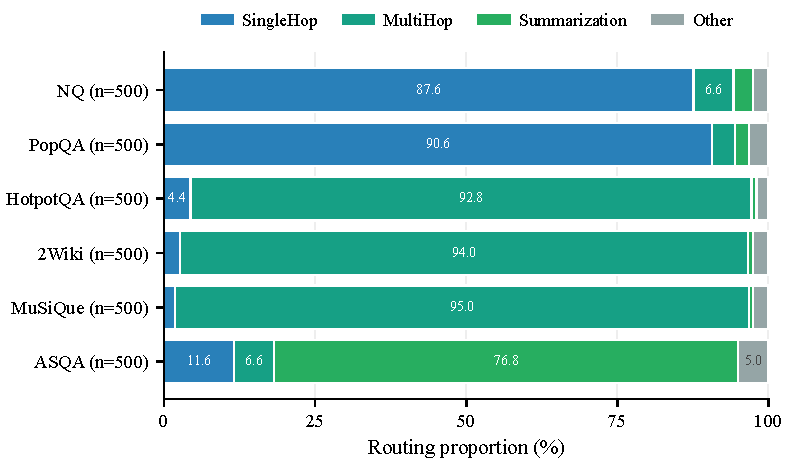
\includegraphics[width=0.92\columnwidth]{figures/fig_routing_dist.pdf}
\caption{Per-dataset routing distribution (Qwen3-8B, full evaluation set of each benchmark). Greeting is 0 on every benchmark: none of the six QA sets contains greeting utterances, so that the L1 regex never fires and 100\% of the benchmark queries are handled by the L2 semantic classifier. The single-hop sets route 87.6--90.6\% to SingleHop, the multi-hop sets route 92.8--95.0\% to MultiHop, and ASQA routes 76.8\% to Summarization.}
\label{fig:routing_dist}
\end{figure}

\paragraph{The distribution matches the division-of-labor design.}
Figure~\ref{fig:routing_dist} reports how queries are routed across the six benchmarks.
The distribution tracks the intent type of each benchmark: NQ and PopQA send 87.6--90.6\% of the queries to SingleHop, the multi-hop sets send 92.8--95.0\% to MultiHop, and ASQA sends 76.8\% to Summarization.
Greeting is zero on every benchmark: the L1 regex never fires, because none of the six QA sets contains greeting utterances, so that 100\% of the benchmark queries are handled by the L2 semantic classifier.
The off-diagonal rates (5--12.4\% on the typed benchmarks, 23.2\% on ASQA) are consistent with the 89.3\% overall accuracy of the L2 classifier reported in Table~\ref{tab:intent}; the higher ASQA off-diagonal rate reflects the fact that its questions are phrased as ambiguous factoids and are sometimes read as multi-hop or single-hop rather than as synthesis.
The distribution also contextualizes the main results: on NQ and PopQA the SingleHop agent handles almost everything, so that the $+4.7$ F1 gain there comes from its hybrid retrieval and reranking rather than from cross-agent routing, whereas on ASQA the 76.8\% of queries that reach the Map-Reduce pipeline of the Summarization agent account for the $+7.2$ F1 outlier, which supports the division-of-labor thesis most directly, since no baseline runs a dedicated aggregation pipeline.

% -------------------------------------------------------------------
\subsection{Multi-hop Depth Boundary}
\label{sec:analysis:depth}

\begin{figure}[t]
\centering
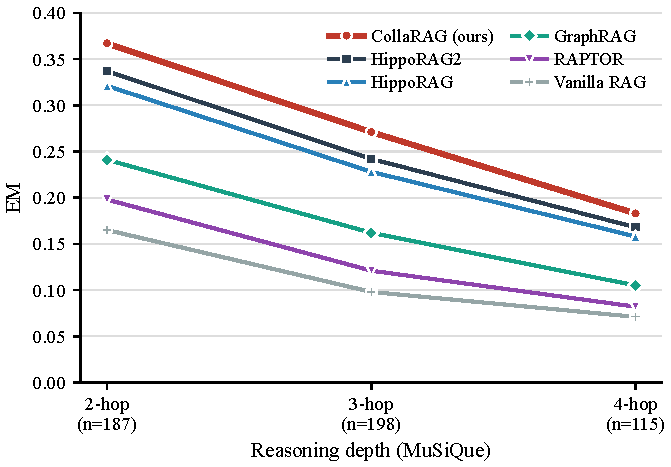
\includegraphics[width=0.96\columnwidth]{figures/fig_hopdepth.pdf}
\caption{EM by reasoning depth on the full answerable MuSiQue evaluation set (MuSiQue-Ans, Qwen3-8B). The lead of \sys{} over HippoRAG2 stays broad at 2-hop and 3-hop ($+3.0$ and $+2.9$ EM) and narrows to $+1.5$ EM at 4-hop, where the reflection budget is exhausted.}
\label{fig:hopdepth}
\end{figure}

Figure~\ref{fig:hopdepth} stratifies MuSiQue-Ans by hop count.
All methods decay sharply with depth; the 2-hop to 4-hop decay of \sys{} (50.1\%) is on par with that of HippoRAG2 (50.1\%), but \sys{} maintains a higher absolute score at every depth.
The lead is widest at 2-hop ($+3.0$ EM) and stays broad at 3-hop ($+2.9$ EM), where the personalized PageRank of HippoRAG2 already covers the two-hop path, and it then narrows to $+1.5$ EM at 4-hop.
The narrowing at 4-hop reveals a capacity limit: the reflection budget ($k_{\max}{=}2$) cannot always repair the deepest evidence chains, which is also why the w/o G-PER ablation costs the least on MuSiQue-Full (3.3 EM) among the multi-hop sets.
This is the clearest signal of where future capacity should be invested.

% -------------------------------------------------------------------
\subsection{Memory Accumulation}
\label{sec:analysis:memory}

\begin{figure}[!htbp]
\centering
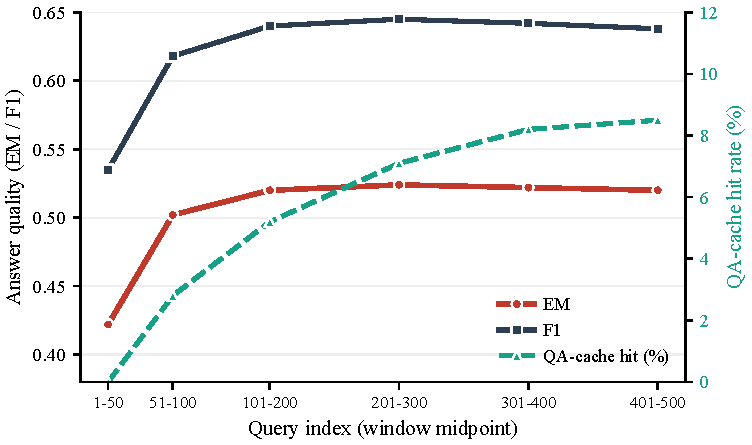
\includegraphics[width=0.96\columnwidth]{figures/fig_memory_curve.pdf}
\caption{Memory accumulation curve on the full HotpotQA evaluation set (Qwen3-8B). As the shared evidence-subgraph overlap cache and the private graph plan templates and gap lessons fill, EM rises from 0.422 (cold) to 0.520 (warm) and the overlap-hit rate climbs to 8.5\%.}
\label{fig:memory_curve}
\end{figure}

Figure~\ref{fig:memory_curve} tracks the performance as queries accumulate in temporal order over the full HotpotQA evaluation set.
EM rises from 0.422 in the first query window (cold start) to 0.520 in the last (warm), a 23.2\% relative gain, and F1 rises from 0.535 to 0.638.
Two mechanisms drive this trend.
The shared evidence-subgraph overlap cache returns high-quality answers for queries whose entity neighborhoods overlap a cached entry, reaching an 8.5\% overlap-hit rate by the final window at zero retrieval or generation cost.
The private layer, comprising graph plan templates and typed gap lessons, fills fastest in the multi-hop bucket, whose entries are also the most frequently reused, so that the same multi-hop routing patterns are reused rather than re-planned and known-missing edges are fetched pre-emptively; this explains why the ablation impact of memory is largest on 2Wiki and HotpotQA (3.0 and 3.1 EM) and smallest on MuSiQue-Full (1.0 EM) (Table~\ref{tab:ablation}).
Growth flattens after approximately 300 queries, i.e.\ within the first few percent of the full evaluation set, which indicates that the bucket capacity ($B_{\max}{=}200$) is well matched to the repetition rate of the workload.

% -------------------------------------------------------------------
\subsection{Hyperparameter Sensitivity}
\label{sec:analysis:hyperparam}

\begin{figure}[!htbp]
\centering
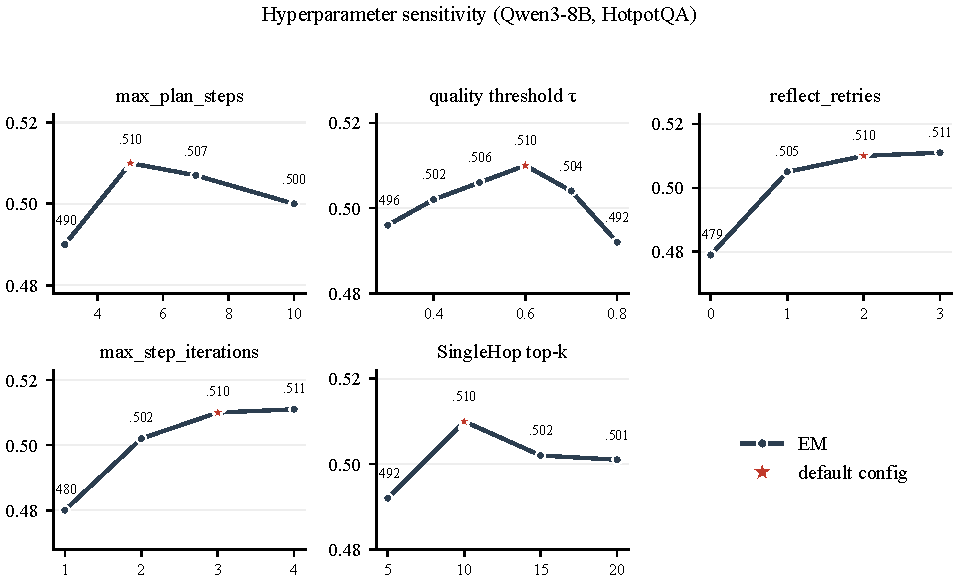
\includegraphics[width=0.8\textwidth]{figures/fig_hyperparam.pdf}
\caption{Hyperparameter sensitivity on the full HotpotQA evaluation set (Qwen3-8B). Each panel sweeps one parameter with the others fixed at the default (starred). All defaults sit on or near the peak, and a one-step perturbation costs at most about 2 EM (typically under 1).}
\label{fig:hyperparam}
\end{figure}

Figure~\ref{fig:hyperparam} sweeps the five governing hyperparameters.
All defaults ($n_{\max}{=}5$, $\tau{=}0.6$, $k_{\max}{=}2$, $j_{\max}{=}3$, and top-$k{=}10$) sit at or within 0.5 EM of the peak, and a one-step perturbation in either direction costs at most about 2 EM (typically under 1), which indicates that the performance of \sys{} does not depend on a narrow optimum.
Plan length peaks at 5 steps: shorter plans under-decompose multi-hop queries, while longer plans let the LLM hallucinate redundant steps, so that the fraction of schema-valid plans declines.
The reflection budget shows diminishing returns: $k{=}0\!\to\!1$ adds 2.6 EM, $1\!\to\!2$ adds 0.5, and $2\!\to\!3$ adds 0.1, and $k_{\max}{=}2$ therefore captures almost all of the available gain at two-thirds of the worst-case cost of $k_{\max}{=}3$.

% -------------------------------------------------------------------
\paragraph{Scaling behavior.}
Comparing the 8B and 32B results, the improvement of \sys{} over the baselines remains stable: the architectural gains from intent routing and G-PER are not ``absorbed'' by a stronger backbone.
This suggests that the contributions of \sys{} are orthogonal to the scaling of LLM capability.

% ===================================================================
% 7. CONCLUSION
% ===================================================================
\section{Conclusion}
\label{sec:conclusion}

We introduced \sys{}, a multi-agent RAG framework built on the principle of graph-grounded division of labor: every routing, reasoning, memory, and capability decision is conditioned on the knowledge graph.
Four innovations drive its effectiveness.
Intent-Aware Query Triage routes queries to specialist agents, which eliminates the one-pipeline-fits-all bottleneck.
G-PER grounds multi-hop reasoning in the knowledge graph through schema-validated planning, frontier-based execution, and structural plus adversarial reflection.
Graph-Grounded Dual-Layer Memory reuses evidence neighborhoods by overlap and stores graph plan templates and gap lessons that feed G-PER, which separates structural learning from cache hits.
Graph-Conditioned Capability Specialization makes the per-agent toolset adaptive to the graph footprint of the query, which supplies a graph-conditioned capability mechanism that prior strategy-level routing lacks.
On six QA benchmarks spanning single-hop, multi-hop, and long-form summarization tasks under two backbone scales, \sys{} achieves the best results among all compared methods, with the largest gains on ASQA ($+7.2$--$+7.4$ F1), where the dedicated Map-Reduce agent is unmatched.
Ablation studies confirm that intent-aware routing is the single most impactful component (a loss of $5.9$ to $12.2$ EM when removed), which validates the division-of-labor hypothesis.

\paragraph{Future work.}
Confidence-based adaptive routing (escalating from SingleHop to MultiHop when the quality is low), inter-agent collaboration for queries that span multiple intent types, and learned tool selection are promising directions.

% ===================================================================
% REFERENCES
% ===================================================================
\bibliographystyle{plainnat}
\clearpage
\bibliography{references}

% ===================================================================
% APPENDIX
% ===================================================================
\appendix

% ===================================================================
% APPENDIX A: PROMPT TEMPLATES
% ===================================================================
\section{Prompt Templates}
\label{app:prompts}

All prompts are centralized in a single module (\texttt{prompts.py}) for reproducibility.
Each template follows a unified structure: \textbf{Role} $\to$ \textbf{Task} $\to$ \textbf{Context} $\to$ \textbf{Format}, with optional \textbf{Few-Shot}, \textbf{COT}, and \textbf{Constraints} blocks.
This appendix lists the core prompts that drive the four innovations.

% -------------------------------------------------------------------
% A.1 Intent Classification
% -------------------------------------------------------------------
\subsection{Intent Classification (\S\ref{sec:triage})}
\label{app:prompt_classify}

\begin{quote}
\small\ttfamily
\textbf{\# Role}\\
You are a query intent classifier for a Retrieval-Augmented Generation system.\\[4pt]
\textbf{\# Task}\\
Classify the following query into exactly one category.\\[4pt]
\textbf{\# Context}\\
Categories and their definitions:\\
- single\_hop: simple factual question answerable from one passage\\
- multi\_hop: requires reasoning across multiple facts, comparison, or exploration\\
- summarization: asks for a summary, overview, or synthesis of information\\
- other: does not fit any above category (e.g.\ weather, jokes, math)\\[4pt]
Query: \{query\}\\[4pt]
\textbf{\# Format}\\
Respond with ONLY the category name (single\_hop / multi\_hop / summarization / other), nothing else.
\end{quote}

% -------------------------------------------------------------------
% A.2 Preprocessor Prompts
% -------------------------------------------------------------------
\subsection{Preprocessor Agent Prompts}
\label{app:prompt_preprocess}

\paragraph{Query Rewrite.}
\begin{quote}
\small\ttfamily
\textbf{\# Role}\\
You are a query rewriting specialist that improves search queries for better retrieval.\\[4pt]
\textbf{\# Task}\\
Rewrite the following query to be clearer, more specific, and self-contained while preserving the original intent.\\[4pt]
\textbf{\# Context}\\
Conversation context: \{context\}\\
Original query: \{query\}\\[4pt]
\textbf{\# Format}\\
Output only the rewritten query, no explanations or prefixes.
\end{quote}

\paragraph{Coreference Resolution.}
\begin{quote}
\small\ttfamily
\textbf{\# Role}\\
You are a coreference resolution specialist that replaces pronouns with explicit entity names.\\[4pt]
\textbf{\# Task}\\
Resolve all pronouns and references in the query using the conversation history.\\[4pt]
\textbf{\# Context}\\
Conversation history: \{history\}\\
Current query: \{query\}\\[4pt]
\textbf{\# Few-Shot}\\
History: ``Who is Albert Einstein?'' | ``He developed the theory of relativity.''\\
Query: Where was he born?\\
Resolved: Where was Albert Einstein born?\\[4pt]
\textbf{\# Format}\\
Output only the resolved query with all pronouns replaced by explicit entities.
\end{quote}

\paragraph{Follow-up Merge.}
\begin{quote}
\small\ttfamily
\textbf{\# Role}\\
You are a conversational query merger that combines follow-up questions with prior context into standalone queries.\\[4pt]
\textbf{\# Task}\\
Rewrite the follow-up question into a single self-contained query that does not depend on prior conversation.\\[4pt]
\textbf{\# Context}\\
Previous question: \{prev\_query\}\\
Previous answer: \{prev\_answer\}\\
Follow-up question: \{query\}\\[4pt]
\textbf{\# Few-Shot}\\
Previous question: What is the capital of France?\\
Previous answer: Paris is the capital of France.\\
Follow-up: What is its population?\\
Self-contained query: What is the population of Paris, the capital of France?\\[4pt]
\textbf{\# Format}\\
Output only the self-contained query, no explanations.
\end{quote}

% -------------------------------------------------------------------
% A.3 SingleHop Agent
% -------------------------------------------------------------------
\subsection{SingleHop Agent Prompt}
\label{app:prompt_singlehop}

\begin{quote}
\small\ttfamily
\textbf{\# Role}\\
You are a precise question-answering assistant that generates answers strictly based on provided evidence.\\[4pt]
\textbf{\# Task}\\
Answer the question using only the given evidence. If the evidence does not contain enough information, say ``I do not know.''\\[4pt]
\textbf{\# Context}\\
Evidence: \{evidence\}\\
Question: \{query\}\\[4pt]
\textbf{\# Format}\\
Provide a concise, factual answer. Use the shortest accurate phrasing --- prefer entity names, numbers, or brief phrases over full sentences.
\end{quote}

% -------------------------------------------------------------------
% A.4 MultiHop Agent (G-PER)
% -------------------------------------------------------------------
\subsection{MultiHop Agent Prompts (G-PER, \S\ref{sec:per})}
\label{app:prompt_multihop}

\paragraph{Plan Generation (schema-constrained graph plan).}
\begin{quote}
\small\ttfamily
\textbf{\# Role}\\
You are a graph-grounded retrieval planner. Decompose a multi-hop query into a plan of graph operations, not free-text sub-queries.\\[4pt]
\textbf{\# Task}\\
1. Identify core entities and the relations the query hinges on.\\
2. Pick a graph operation per step: ``link'' (resolve/confirm an entity), ``traverse'' (follow a relation), ``attribute'' (look up a fact), or ``aggregate'' (merge facts across entities).\\
3. Order steps with dependencies.\\
4. Suggest retrieval tools per step.\\[4pt]
\textbf{\# Context}\\
Available tools: \{tool\_descriptions\}\\
Known relation types in the KG (schema): \{schema\}\\
Query: \{query\}\\[4pt]
\textbf{\# Format}\\
Output a JSON list of steps: \{``op'': ``link$|$traverse$|$attribute$|$aggregate'', ``entity'': $\ldots$, ``relation'': $\ldots$, ``target'': $\ldots$, ``step'': $\ldots$, ``tools\_hint'': [$\ldots$], ``depends\_on'': [$\ldots$]\}. Only use relation types from the schema; use null when unknown.\\[4pt]
\textbf{\# Few-Shot}\\
Query: ``Compare the populations of Tokyo and New York''\\
Plan: [\{``op'':``attribute'',``entity'':``Tokyo'',``relation'':``population'',``target'':null,``step'':``Find Tokyo's population'',``tools\_hint'':[``hybrid\_search''],``depends\_on'':[]\}, \{``op'':``attribute'',``entity'':``New York'',``relation'':``population'',``target'':null,``step'':``Find New York's population'',``tools\_hint'':[``hybrid\_search''],``depends\_on'':[]\}, \{``op'':``aggregate'',``entity'':null,``relation'':null,``target'':null,``step'':``Compare the two populations'',``tools\_hint'':[],``depends\_on'':[0,1]\}]
\end{quote}

Each step is then validated against the KG schema before execution (\S\ref{sec:per}, Eq.~\ref{eq:validate}); steps whose relation is not in the schema or whose entity is unknown are degraded to free sub-queries rather than dropped.

\paragraph{Step Execution (ReAct, frontier-budgeted).}
\begin{quote}
\small\ttfamily
\textbf{\# Role}\\
You are a retrieval execution agent using the ReAct paradigm.\\[4pt]
\textbf{\# Task}\\
Execute step \{step\_num\} of the plan:\\
1. Analyze what information is needed\\
2. Choose the most appropriate tool\\
3. Formulate precise tool inputs\\
4. Evaluate the output --- if insufficient, try a different tool or refined query\\
5. Summarize key findings once enough evidence is gathered\\[4pt]
\textbf{\# Context}\\
Plan step: \{step\_description\}\\
Original query: \{query\}\\
Previous steps evidence: \{previous\_evidence\}\\
Available tools: \{tool\_descriptions\}\\[4pt]
\textbf{\# COT}\\
Thought: $\ldots$\\
Action: tool\_name\\
Action Input: \{``param'': ``value''\}\\
Observation: ($\ldots$)\\
\ldots\ (repeat if needed)\\
Step Result: $\ldots$\\[4pt]
\textbf{\# Format}\\
Follow the COT format strictly. Begin with ``Thought:'' and end with ``Step Result:''.
\end{quote}

Steps draw iterations from a shared global frontier budget $J$ (Eq.~\ref{eq:exec}); a step that emits a Step Result early donates its unused iterations to downstream steps.

\paragraph{Reflection (structural-completeness repair).}
\begin{quote}
\small\ttfamily
\textbf{\# Role}\\
You are a graph-grounded evidence auditor that turns structural evidence gaps into targeted repair actions.\\[4pt]
\textbf{\# Task}\\
Given typed structural gaps already detected by the completeness checker, produce a precise repair per gap. Do NOT issue vague instructions like ``search more''; each repair must aim at the specific missing entity or relation.\\[4pt]
\textbf{\# Context}\\
Original query: \{query\}\\
Gathered evidence: \{step\_results\}\\
Detected structural gaps (each is a specific missing edge/attribute): \{gaps\}\\[4pt]
\textbf{\# Format}\\
Output a JSON list of repairs: [\{``gap'': $\ldots$, ``repair\_query'': $\ldots$, ``tools\_hint'': [$\ldots$], ``target\_entities'': [$\ldots$]\}]. Output [] if no gaps.
\end{quote}

Gaps are produced by the structural-completeness checker $\Gamma$ (Eq.~\ref{eq:reflect}), which infers the required evidence shape from the query (comparison, bridge, or attribute) and diffs it against the gathered subgraph, emitting typed gaps (\texttt{missing\_attribute}, \texttt{missing\_path}, and \texttt{missing\_relation}).

\paragraph{Adversarial Probe (graph-level contradiction check).}
\begin{quote}
\small\ttfamily
\textbf{\# Role}\\
You are an adversarial fact-checker that probes the KG for relations contradicting a draft answer.\\[4pt]
\textbf{\# Task}\\
For each atomic claim in the draft answer, decide whether the gathered evidence or KG contains a competing or contradicting relation that the answer ignored. A claim is ``contested'' if a plausible alternative relation exists.\\[4pt]
\textbf{\# Context}\\
Query: \{query\}\\
Draft answer: \{draft\_answer\}\\
Evidence triples (subject, predicate, object): \{triples\}\\[4pt]
\textbf{\# Format}\\
Output JSON: \{``verdict'': ``confirmed$|$contested$|$unsupported'', ``contested\_claims'': [$\ldots$], ``reason'': $\ldots$\}.
\end{quote}

\paragraph{Synthesis.}
\begin{quote}
\small\ttfamily
\textbf{\# Role}\\
You are an evidence synthesis specialist that produces comprehensive answers from multi-step retrieval results.\\[4pt]
\textbf{\# Task}\\
Synthesize all gathered evidence into a final answer:\\
1. Collect and organize all relevant facts\\
2. Resolve any conflicts between different evidence sources\\
3. Construct a coherent answer that addresses every aspect of the query\\
4. Verify that no key aspect is left unanswered\\[4pt]
\textbf{\# Context}\\
Query: \{query\}\\
Evidence from plan execution: \{all\_evidence\}\\[4pt]
\textbf{\# Format}\\
Provide a comprehensive answer that integrates facts from all the evidence. Cite specific facts. Be accurate and do not hallucinate beyond what the evidence supports.
\end{quote}

% -------------------------------------------------------------------
% A.5 Summarization Agent
% -------------------------------------------------------------------
\subsection{Summarization Agent Prompts}
\label{app:prompt_summarization}

\paragraph{Map (per-chunk extraction).}
\begin{quote}
\small\ttfamily
\textbf{\# Role}\\
You are an information extraction specialist that identifies key facts relevant to a query.\\[4pt]
\textbf{\# Task}\\
Extract key information from the given passage that is relevant to answering the query.\\[4pt]
\textbf{\# Context}\\
Query: \{query\}\\
Passage: \{text\}\\[4pt]
\textbf{\# Format}\\
Output a concise list of key facts and information extracted from the passage. Include only information relevant to the query.
\end{quote}

\paragraph{Reduce (synthesis).}
\begin{quote}
\small\ttfamily
\textbf{\# Role}\\
You are a summarization specialist that synthesizes extracted information into coherent summaries.\\[4pt]
\textbf{\# Task}\\
Combine the following extracted information fragments into a comprehensive, well-structured summary that answers the query.\\[4pt]
\textbf{\# Context}\\
Query: \{query\}\\
Extracted information: \{summaries\}\\[4pt]
\textbf{\# Format}\\
Provide a coherent summary that integrates all relevant extracted information. Organize it logically and avoid redundancy.
\end{quote}

% -------------------------------------------------------------------
% A.6 Reasoning Tool Prompts
% -------------------------------------------------------------------
\subsection{Reasoning Tool Prompts}
\label{app:prompt_tools}

\paragraph{Sub-query Decomposition.}
\begin{quote}
\small\ttfamily
\textbf{\# Role}\\
You are a query decomposition specialist that breaks complex questions into simpler sub-questions.\\[4pt]
\textbf{\# Task}\\
Decompose the following complex query into simpler, independent sub-queries that can each be answered separately.\\[4pt]
\textbf{\# Context}\\
Query: \{query\}\\[4pt]
\textbf{\# Few-Shot}\\
Query: ``What are the similarities and differences between photosynthesis and cellular respiration?''\\
Sub-queries: [``What is photosynthesis and how does it work?'', ``What is cellular respiration and how does it work?'', ``What do photosynthesis and cellular respiration have in common?'', ``How do photosynthesis and cellular respiration differ?'']\\[4pt]
\textbf{\# Format}\\
Return a JSON list of strings. Maximum 4 sub-queries.
\end{quote}

\paragraph{Entity Extraction.}
\begin{quote}
\small\ttfamily
\textbf{\# Role}\\
You are a named entity recognition specialist for knowledge graph queries.\\[4pt]
\textbf{\# Task}\\
Extract all named entities and key concepts from the query that could be used to search a knowledge graph.\\[4pt]
\textbf{\# Context}\\
Query: \{query\}\\[4pt]
\textbf{\# Few-Shot}\\
Query: ``What is the relationship between Einstein and the University of Zurich?''\\
JSON: \{``entities'': [``Einstein'', ``University of Zurich'']\}\\[4pt]
\textbf{\# Format}\\
Return a JSON object with a single key ``entities'' containing a list of strings. Include only meaningful entities, not common words.
\end{quote}

\paragraph{Answer Verification.}
\begin{quote}
\small\ttfamily
\textbf{\# Role}\\
You are a factual verification specialist that checks whether an answer is supported by evidence.\\[4pt]
\textbf{\# Task}\\
Verify the draft answer against the provided evidence:\\
1. Identify each factual claim in the draft answer\\
2. For each claim, check if it is directly supported by the evidence\\
3. Flag any claim that is unsupported, contradicted, or hallucinated\\
4. Produce a final verdict: verified, partially\_verified, or rejected\\[4pt]
\textbf{\# Context}\\
Question: \{query\}\\
Draft answer: \{draft\_answer\}\\
Evidence: \{evidence\}\\[4pt]
\textbf{\# Format}\\
Return a JSON object: \{``verdict'': ``verified|partially\_verified|rejected'', ``supported\_claims'': [\ldots], ``unsupported\_claims'': [\ldots], ``reason'': ``\ldots''\}
\end{quote}

% ===================================================================
% APPENDIX B: FULL TOOL INVENTORY
% ===================================================================
\section{Full Tool Inventory}
\label{app:tools}

The 34 shared tools span ten functional categories.
Table~\ref{tab:tool_full} lists each tool with its inputs, outputs, LLM dependency, and the agents that may invoke it (per the tool-permission matrix in Table~\ref{tab:tool_matrix}).

\begin{table*}[t]
\centering
\small
\begin{tabular}{@{}lllcc@{}}
\toprule
\textbf{Category} & \textbf{Tool Name} & \textbf{Function} & \textbf{LLM?} & \textbf{Agents} \\
\midrule
\multirow{6}{*}{Retrieval}
  & \tool{vector\_search}        & Dense embedding similarity search over a FAISS index         & No  & SH, MH, SM \\
  & \tool{bm25\_search}          & Sparse lexical search via a BM25 inverted index              & No  & SH, MH, SM \\
  & \tool{hybrid\_search}        & RRF fusion of dense + sparse, with optional rerank              & No  & SH, MH, SM, OT \\
  & \tool{graph\_neighbors}      & $k$-hop neighborhood expansion from seed entities          & No  & SH, MH \\
  & \tool{graph\_path\_search}   & Shortest path between two entities in the KG               & No  & MH \\
  & \tool{graph\_community\_search} & Community-level subgraph retrieval                       & No  & MH, SM \\
\midrule
\multirow{3}{*}{Entity}
  & \tool{entity\_extract}       & Extract named entities from a query (LLM-based NER)          & Yes & SH, MH, SM, OT \\
  & \tool{relation\_extract}     & Extract (subject, predicate, object) triples from a query    & Yes & MH \\
  & \tool{entity\_link}          & Map extracted entity names to canonical graph nodes        & Yes & SH, MH \\
\midrule
\multirow{3}{*}{Reasoning}
  & \tool{sub\_query\_decompose} & Decompose a complex query into $\le$4 independent sub-queries & Yes & MH \\
  & \tool{assess\_evidence}      & Score evidence completeness for reflection ($\hat{q}\in[0,1]$) & No & SH, MH \\
  & \tool{rerank}                & Cross-encoder reranking of retrieved chunks                & No  & SH, MH, SM \\
\midrule
\multirow{3}{*}{Preprocessing}
  & \tool{query\_rewrite}        & Expand and clarify a query for better retrieval               & Yes & PP \\
  & \tool{coreference\_resolve}  & Replace pronouns with explicit entity references            & Yes & PP \\
  & \tool{followup\_merge}       & Merge a follow-up question with prior context into a standalone query & Yes & PP \\
\midrule
\multirow{6}{*}{Memory}
  & \tool{read\_shared\_memory}   & Read the QA cache, routing stats, and entity aliases       & No  & All \\
  & \tool{write\_shared\_memory} & Write to the shared QA cache / routing stats / entity aliases & No  & SH, MH, SM \\
  & \tool{read\_agent\_memory}    & Read per-agent per-intent experiential memory (JSONL)      & No  & SH, MH, SM, OT \\
  & \tool{write\_agent\_memory}   & Write to per-agent per-intent experiential memory (JSONL)  & No  & SH, MH, SM, OT \\
  & \tool{read\_session\_context} & Read in-process dialogue history                           & No  & PP, MH \\
  & \tool{write\_session\_context} & Write a QA turn to in-process dialogue history             & No  & PP, MH \\
\midrule
\multirow{2}{*}{Web}
  & \tool{web\_search}           & DuckDuckGo / SerpAPI external search                       & No  & OT \\
  & \tool{web\_fetch}            & Fetch and parse a single URL                                & No  & OT \\
\midrule
\multirow{2}{*}{File I/O}
  & \tool{save\_to\_file}        & Persist intermediate results to disk                        & No  & SH, MH, SM, OT \\
  & \tool{load\_from\_file}      & Load previously saved results                               & No  & SH, MH, SM, OT \\
\midrule
\multirow{3}{*}{Verification}
  & \tool{answer\_verify}        & Verify a draft answer against evidence (supported or rejected)  & Yes & SH, MH \\
  & \tool{claim\_decompose}      & Decompose text into atomic, independently verifiable claims & Yes & MH \\
  & \tool{source\_attribution}   & Trace each answer claim back to its evidence chunk\_id     & Yes & MH, SM \\
\midrule
\multirow{2}{*}{Graph Analysis}
  & \tool{graph\_subgraph\_extract} & Extract a focused $k$-hop subgraph around seed entities   & Yes & MH \\
  & \tool{graph\_statistics}     & Return graph-level statistics (nodes, edges, hubs, density)& No  & MH \\
\midrule
\multirow{4}{*}{Evidence}
  & \tool{temporal\_filter}      & Filter evidence chunks by a year or date range                  & No  & MH \\
  & \tool{evidence\_dedup}       & Deduplicate chunks by Jaccard token similarity             & No  & SH, MH, SM \\
  & \tool{chunk\_summarize}      & Compress a chunk while preserving query-relevant facts     & Yes & MH, SM \\
  & \tool{confidence\_calibrate} & Multi-signal answer confidence score ($\in[0,1]$)          & No  & SH, MH, SM, OT \\
\bottomrule
\end{tabular}
\caption{Full inventory of the 34 shared tools. ``LLM?'' indicates whether the tool internally calls the backbone LLM. ``Agents'' lists which specialists may invoke each tool (PP denotes the Preprocessor, SH SingleHop, MH MultiHop, SM Summarization, and OT Other). Tools that are not assigned to an agent are invisible to it, which is enforced by the \texttt{ToolSetBuilder} and the tool-permission matrix (Table~\ref{tab:tool_matrix}).}
\label{tab:tool_full}
\end{table*}

\end{document}
